\chapter{Two-dimensional finite-volume methods}
\label{chp-2d-fv}
In Chapter \ref{chp-1d-fv}, we tackled the problem of solving the one-dimensional linear
advection equation using the finite-volume method based on PPM.
In this Chapter, we are interested in solving the two-dimensional linear
advection equation using the finite-volume method. This step plays a key role in this work,
since as we shall see in Chapter  \ref{chp-cs-fv}, the solution of the linear
advection equation on the cubed-sphere boils down to solving one two-dimensional linear
advection equations at each cube face with interpolation between the adjacent panels.

A natural way to derive a finite-volume method for the two-dimensional linear
advection equation would be to extend the PPM for two dimensions. Indeed, a piecewise bi-parabolic extension of PPM
was proposed by \citet{rancic:1992} using a semi-lagrangian temporal discretization. 
However, the major problem of this method is its quite expensive computational cost.
A popular alternative, and usually computationally cheaper, is to use dimension-splitting methods.
These schemes replace two-dimensional problem with a sequence of one-dimensional problems.
For instance, we can solve the two-dimensional linear advection equation by solving a sequence
one-dimensional linear advection equations using the PPM  from Chapter \ref{chp-1d-fv}.
Further, we could, in principle, use any numerical method that solves the one-dimensional linear advection. 
A comparison between two-dimension and dimension splitting semi-lagrangian schemes on the plane has been investigated by \citet{chen:2017}
using the PPM as the one-dimensional solver and distorted two-dimensional grids.
Their major conclusion is that the dimension splitting schemes are more sensitive to grid distortions
but it is computationally cheaper and more accurate than their two-dimensional methods, 
specially considering large CFL numbers.

The main aim of this chapter is to give a detailed description of the dimension
splitting method proposed by \citet{lin:1996}, which is currently employed in the FV3 dynamical core,
applied to the two-dimensional linear advection equation using the one-dimensional
finite-volume schemes from Chapter \ref{chp-1d-fv}.
Similarly to Chapter \ref{chp-1d-fv}, we start this Chapter 
start with a review of the two-dimensional advection equation in
the integral form in Section \ref{sec-adv2d}, 
and in Section \ref{sec:fv-2d} we set the framework of
general two-dimensional finite-volumes schemes.
Section \ref{sec-dsplit} presents the dimension splitting method and 
numerical experiments are shown in Section \ref{sec-ds-exp}.

\section{Two-dimensional advection equation in integral form}
\label{sec-adv2d}
Let us consider a $\mathcal{C}^1$ velocity field given by
$\boldsymbol{u}: \mathbb{R}^2 \to \mathbb{R}^2$,  $\boldsymbol{u}=(u,v)$, where
$u$ is the velocity in $x$-direction and $v$ is the velocity in $x$ and $y$ direction. 
The two-dimensional advection equation in the differential form in 
a domain $\Omega=[a,b]\times[c,d] \subset \mathbb{R}^2$
associated to the velocity field $\boldsymbol{u}$ is given by:
\begin{equation}
\label{sec-adv2d:eq1}
\frac{\partial q}{\partial t}(x, y, t) +
\nabla \cdot (q\boldsymbol{u})(x, y, t)
= 0, \quad \forall (x, y, t) \in \Omega^{\mathrm{o}}
 \times ]0, +\infty[,
\footnote{$\Omega^{\mathrm{o}}$ denotes the interior of $\Omega$. 
	Namely, $\Omega^{\mathrm{o}} = ]a,b[ \times ]c,d[$.}
\end{equation}
where $\nabla \cdot (q\boldsymbol{u})$ is the spatial divergence
\begin{equation}
	\label{sec-adv2d:eqdiv}
	\nabla \cdot (q\boldsymbol{u})(x, y, t) =  
	\frac{\partial (uq)}{\partial x}(x, y, t) + \frac{\partial (vq)}{\partial y}(x, y, t).
\end{equation}
We recall that we say the $u$ is \textbf{non-divergent} if $\nabla \cdot \boldsymbol{u}=0$. 
A classical or strong solution to the two-dimensional advection equation is a 
$\mathcal{C}^1$ function ${q}$ satisfying Equation \eqref{sec-adv2d:eq1}.
As we did in Section \ref{chp2-sec1}, our goal is to deduce an
integral form of Equation \eqref{sec-adv2d:eq1}.
Thus, let us consider  $[x_1,x_2] \times [y_1, y_2]
\subset \Omega^{\mathrm{o}}$ and $[t_1,t_2] \subset [0, +\infty[$.
Integrating Equation $\eqref{sec-adv2d:eq1}$ over 
$[x_1,x_2] \times [y_1, y_2]$ yields:
\begin{align}
	\label{sec-adv2d:eq2}
	\frac{d}{d t} \bigg(\int_{x_1}^{x_2} \int_{y_1}^{y_2}
	{q}(x, y, t) \,dx \,dy \bigg)=
	&-\int_{y_1}^{y_2} \bigg({(uq)}(x_2, y, t)
	-{(uq)}(x_1, y, t) \bigg) \,dy \\ \nonumber
	&-\int_{x_1}^{x_2} \bigg({(vq)}(x, y_2, t)
	-{(vq)}(x, y_1, t) \bigg) \,dx.
\end{align}
Integrating Equation \eqref{sec-adv2d:eq2} over the time interval $[t_1,t_2]$, 
we have:
\begin{align}
	\label{sec-adv2d:eq3}
	\int_{x_1}^{x_2} \int_{y_1}^{y_2}
	{q}(x, y, t_{n+1}) \,dx \,dy = &\int_{x_1}^{x_2} \int_{y_1}^{y_2}
	{q}(x, y, t_n) \,dx \,dy \\ \nonumber
	&-\int_{t_1}^{t_2} \int_{y_1}^{y_2} \bigg({(uq)}(x_2, y, t)
	-{(uq)}(x_1, y, t) \bigg) \,dy \,dt\\ \nonumber
	&-\int_{t_1}^{t_2} \int_{x_1}^{x_2} \bigg({(vq)}(x, y_2, t)
	-{(vq)}(x, y_1, t) \bigg) \,dx \,dt.
\end{align}
Equation \eqref{sec-adv2d:eq3} is the integral form of Equation 
\eqref{sec-adv2d:eq1}. We say that ${q}$ is a weak
solution to the advection equation \eqref{sec-adv2d:eq1} if ${q}$
satisfies the integral form \eqref{sec-adv2d:eq3}, 
$\forall [x_1,x_2]\times[y_1,y_2] \subset \Omega^{\mathrm{o}}$ and 
$\forall [t_1,t_2] \subset [0,+\infty[$.
Similarly to Section \ref{chp2-sec1}, these problems are equivalent
when  ${q}$ is a $\mathcal{C}^1$ function.
We consider an initial condition ${q_0}$,
${q}(x,y,0) =  {q_0}(x,y)$, $\forall (x,y) \in \Omega$.
Boundary conditions will be assumed bi-periodic.
%At last, the matrix $\alpha D{f}(q) + \beta D{g}(q)$ is assumed to have
%real eigenvalues and be diagonalizable
%$\forall q \in \mathbb{R}^m , \forall \alpha, \beta \in \mathbb{R}$
%\citep{leveque:1990}, so that we have a hyperbolic conservation law.
Therefore, we are again dealing with a Cauchy problem. 
%Besides that, the two-dimensional advection equation is a hyperbolic PDE.

To move in the direction of a discrete version of Equation \eqref{sec-adv2d:eq3},
let us discretize the domain $D = \Omega \times [0,T]$ following 
the notations of Section \ref{chp2-sec1}.
Given a positive integer $N_T$, we define the time step 
$\Delta t = \frac{T}{N_T}$, $t_n = n \Delta t$, for $n = 0, 1 ,\cdots, N_T$.
The spatial discretization is constructed through an uniformly spaced partition of $\Omega$ given by:
\begin{align}
	[a,b] &= \bigcup_{i=1}^N X_i, 
	\text{ where } X_i= [x_{i-\frac{1}{2}}, x_{i+\frac{1}{2}}] \text{ and } 
	a = x_{\frac{1}{2}} < x_{\frac{3}{2}} < \cdots < x_{N-\frac{1}{2}} < x_{N+\frac{1}{2}} = b, \\
	[c,d] &= \bigcup_{j=1}^M Y_j, 
\text{ where } Y_j= [y_{j-\frac{1}{2}}, y_{j+\frac{1}{2}}] \text{ and } 
	c = y_{\frac{1}{2}} < y_{\frac{3}{2}} < \cdots < y_{M-\frac{1}{2}} < y_{M+\frac{1}{2}} = d, \\
    \Omega &=  \bigcup_{i=1}^N \bigcup_{j=1}^M \Omega_{ij}, \text{ where } \Omega_{ij} = X_i \times Y_j.
\end{align}
The regions $\Omega_{ij}$ are known as control volumes or cells. \index{Control volume}
Similarly to  Chapter \ref{chp-1d-fv} we employ the notations
$\Delta x = x_{i+\frac{1}{2}} - x_{i-\frac{1}{2}}$,
$\Delta y = y_{j+\frac{1}{2}} - y_{j-\frac{1}{2}}$ 
and $x_i = \frac{1}{2}(x_{i+\frac{1}{2}} + x_{i-\frac{1}{2}})$
$y_j = \frac{1}{2}(y_{j+\frac{1}{2}} + y_{j-\frac{1}{2}})$, $\forall i = 1, \cdots, N$, 
$\forall j = 1, \cdots, M$,
to define the control volume lengths and centroids, respectively.
Finally, we denote by ${Q}_{ij}(t)$ as the
average values of state variable at time $t$
in the control volume $\Omega_{ij}$, that is:
\begin{equation}
	\label{sec-adv2d:eq4}
	{Q}_{ij}(t) = \frac{1}{\Delta x \Delta y}
	\int_{x_{i-\frac{1}{2}}}^{x_{i+\frac{1}{2}}} \int_{y_{j-\frac{1}{2}}}^{y_{j-\frac{1}{2}}} {q}(x,y,t) \,dx.
\end{equation}
Substituting $t_1, t_2, x_1, x_2, y_1$ and $y_2$ by 
$t_{n}, t_{n+1}, x_{i-\frac{1}{2}}, x_{i+\frac{1}{2}}, y_{j-\frac{1}{2}}, y_{j+\frac{1}{2}}$,
respectively, in Equation \eqref{sec-adv2d:eq3}, we obtain:
\begin{align}
	\label{sec-adv2d:eq5}
	{Q}_{ij}(t_{n+1})  = {Q}_{ij}(t_{n})
	&- \frac{\Delta t}{\Delta x \Delta y}
	\delta _x \bigg( \frac{1}{\Delta t}
	\int_{t_1}^{t_2} \int_{y_{j-\frac{1}{2}}}^{y_{j+\frac{1}{2}}} 
	{(uq)}(x_{i}, y, t)
	\,dy \,dt \bigg) \\ \nonumber
	&- \frac{\Delta t}{\Delta x \Delta y}
	\delta _y \bigg( \frac{1}{\Delta t}
	\int_{t_1}^{t_2} \int_{x_{i-\frac{1}{2}}}^{x_{i+\frac{1}{2}}} 
	{(vq)}(x, y_{j}, t)
	\,dx \,dt \bigg),
\end{align}
where we are using the centered finite-difference notation:
\begin{align}
	\label{sec-adv2d:eq6}
	\delta_x {h}(x_i,y, t) = 
	{h}(x_{i+\frac{1}{2}}, y, t) - 
	{h}(x_{i-\frac{1}{2}}, y, t), \\
	\delta_y {h}(x, y_j,t) = 
    {h}(x, y_{j+\frac{1}{2}},t) - 
    {h}(x, y_{j-\frac{1}{2}},t),
\end{align}
for any function ${h}$. The Equation \eqref{sec-adv2d:eq5} is useful to
motivate two-dimensional finite-volume schemes, as we shall see in the next section.

\section{The finite-volume approach}
\label{sec:fv-2d}
This Section is basically an extension to two dimensions of the concepts presented in Section \ref{chp2-sec2}.
We introduce the following spaces of bi-periodic functions:
\begin{align*}
	\mathcal{F}(\mathbb{T}^2) &= \{q:\mathbb{R}^2 \to \mathbb{R};
	\quad q(x+b-a,y) = q(x,y), \quad q(x,y+d-c) = q(x,y),\quad \forall (x,y) \in \mathbb{R}^2\},\\
	\mathcal{F}(\mathbb{T}^2_{T}) &= \{q:\mathbb{R}^2\times[0,T]\to \mathbb{R};\quad q(\cdot,\cdot,t) \in \mathcal{F}(\mathbb{T}^2), \quad \forall t \in [0,T]\},\\
	\mathcal{C}^k(\mathbb{T}^2_{T}) &= \{q\in \mathcal{C}^k(\mathbb{R}^2\times[0,T]): q \in \mathcal{F}(\mathbb{T}^2_{T})\}.
\end{align*}
where we are using the notation $\mathbb{T}^2_{T} = \mathbb{T}^2\times[0,T]$ and $\mathbb{T}^2 = [a,b] \times [c,d]$ denotes the torus of lengths $b-a$ and $d-c$.
We are using the notation $\mathbb{T}^2$ since we may think of bi-periodic functions as functions defined on the torus of lengths $b-a$ and $d-c$.
Whenever we use the notation $\mathbb{T}^2$, $a, b, c$ and $d$ will be implicitly defined.
We also introduce the following the locally integrable periodic functions:
\begin{align*}
	L^p_{\text{loc}}(\Omega) &= \{q:\Omega\to \mathbb{R};\quad \int_{K} |q(x,y)|^p\,dx\,dy  < +\infty, \quad \text{for all compact sets } K \subset \Omega\},\\
	{L}^{p}_{\text{loc}}(\mathbb{T}^2) &= \{q\in \mathcal{F}(\mathbb{T}^2): \quad  q \in L^p_{\text{loc}}(\mathbb{R}^2)\},\\
	{L}^{p,x,y}_{\text{loc}}(\mathbb{T}^2_{T}) &= \{q\in \mathcal{F}(\mathbb{T}^2_{T}): \forall t \in [0,T], \quad q(\cdot,\cdot,t) \in L^p_{\text{loc}}(\mathbb{R}^2)\},\\
	{L}^{p,y,t}_{\text{loc}}(\mathbb{T}^2_{T}) &= \{q\in \mathcal{F}(\mathbb{T}^2_{T}): \forall x \in \mathbb{R},\quad q(x,\cdot,\cdot) \in L^p_{\text{loc}}(\mathbb{R}\times [0,T])\},\\
	{L}^{p,x,t}_{\text{loc}}(\mathbb{T}^2_{T}) &= \{q\in \mathcal{F}(\mathbb{T}^2_{T}): \forall y \in \mathbb{R},\quad q(\cdot,y,\cdot) \in L^p_{\text{loc}}(\mathbb{R}\times [0,T])\}.\\
\end{align*}

\subsection{Discretization of the problem}
The problem of two-dimensional advection equation in the integral form 
presented Section \ref{sec-adv2d} is written in a concise way in Problem \ref{chp3-sec2-prob1}.
\begin{prob}
	\label{chp3-sec2-prob1}
	Given an initial condition ${q}_0\in {L}^{1}_{\text{loc}}(\mathbb{T}^2) \cap {L}^{2}_{\text{loc}}(\mathbb{T}^2)$ and
	a velocity function $u \in {L}^{2,y,t}_{\text{loc}}(\mathbb{T}^2_{T})$ in the $x$-direction, 
	a velocity function $v \in {L}^{2,x,t}_{\text{loc}}(\mathbb{T}^2_{T})$ in the $y$-direction, 
 	we would like to find a weak solution 
 	${q} \in {L}^{1,x,y}_{\text{loc}}(\mathbb{T}^1_{T}) \cap {L}^{2,x,t}_{\text{loc}}(\mathbb{T}^2_{T}) \cap {L}^{2,y,t}_{\text{loc}}(\mathbb{T}^2_{T})$
	of the two-dimensional advection equation in the integral form:
	\begin{align*}
		\int_{x_1}^{x_2} \int_{y_1}^{y_2}
		{q}(x, y, t) \,dx \,dy = &\int_{x_1}^{x_2} \int_{y_1}^{y_2}
		{q}(x, y, t) \,dx \,dy \\ \nonumber
		&-\int_{t_1}^{t_2} \int_{y_1}^{y_2} \bigg({(uq)}(x_2, y, t)
		-{(uq)}(x_1, y, t) \bigg) \,dy \,dt\\ \nonumber
		&-\int_{t_1}^{t_2} \int_{x_1}^{x_2} \bigg({(vq)}(x, y_2, t)
		-{(vq)}(x, y_1, t) \bigg) \,dx \,dt.
	\end{align*}
	$\forall [x_1, x_2]\times [y_1, y_2] \times[t_1, t_2] \subset [a,b] \times [c,d] \times[0,T]$, 
	and ${q}(x, y, 0) = {q}_0(x, y)$, $\forall (x, y) \in [a,b] \times [c,d]$.
\end{prob}
For Problem \ref{chp3-sec2-prob1}, the total mass in $\Omega$ is defined by: 
\begin{equation}
	{M}_{\Omega}(t) = \int_{\Omega} {q}(x,y,t) \,dx \,dy , \quad \forall t \in [0,T],
\end{equation}
and is conserved within time: 
\begin{equation}
	{M}_{\Omega}(t) = {M}_{\Omega}(0), \quad \forall t \in [0,T].
\end{equation}
considering a discretization of the domain $[a,b] \times [0,T]$. 
Similar to Definitions \ref{chp2-def-2dgrid} and \ref{chp2-def-dxtimegrid},
we introduce the concepts of $(\Delta x,\Delta y)$-grid and $(\Delta x, \Delta y,\Delta t, \lambda_x,\lambda_y)$ discretization.
\begin{definition}[$(\Delta x,\Delta y)$-grid]
	\label{chp2-def-2dgrid}
	Given $[a,b]\times [c,d]$ and positive real numbers $\Delta x$ and $\Delta y$ such that $\Delta x = (b-a)/N$, 
	$\Delta y = (d-c)/M$, for positive integers $N$ and $M$,
	we say that a $(N,M)$-tuple $\mathcal{D}=(\Omega_{ij})_{i=1,\cdots,N,j=1,\cdots,M}$ is a $(\Delta x, \Delta y)$-grid for $[a,b]\times [c,d]$ if
	$\Omega_{ij} = [x_{i-\frac{1}{2}}, x_{i+\frac{1}{2}}]\times [y_{j-\frac{1}{2}}, y_{j+\frac{1}{2}}]$, 
	$a = x_{\frac{1}{2}} < x_{\frac{3}{2}} < \cdots < x_{N-\frac{1}{2}} < x_{N+\frac{1}{2}} = b$,
	$c = y_{\frac{1}{2}} < y_{\frac{3}{2}} < \cdots < y_{M-\frac{1}{2}} < y_{M+\frac{1}{2}} = d$,
	$\Delta x = x_{i+\frac{1}{2}}-x_{i-\frac{1}{2}}$, 	$\Delta y = y_{j+\frac{1}{2}}-y_{j-\frac{1}{2}}$.
	Each $\Omega_{ij}$ is called control volume or cell.
\end{definition}
\begin{remark}
	We may define the cells $\Omega_{ij}$ for $i$ outside of the range $1,\cdots, N$ or $j$ outside of the range $1,\cdots, M$  by 
	$\Omega_{ij} = [a+(i-1)\Delta x,a+i\Delta x]\times [c+(j-1)\Delta x,c+j\Delta x]$.  These cells are called ghost cells.
\end{remark}
\begin{definition}[$(\Delta x,\Delta y,\Delta t, \lambda_x, \lambda_y)$-discretization]
	\label{chp2-def-dxdytimegrid}
	Given $[a,b]\times[c,d]\times [0,T]$ and positive real numbers $\Delta x$ $\Delta y$ and $\Delta t$, we say that $(\mathcal{D},\mathcal{T})$ is a
	$(\Delta x,\Delta y,\Delta t, \lambda_x, \lambda_y)-$discretization of $[a,b]\times[c,d]\times [0,T]$ if $\Omega$ is a $(\Delta x,\Delta y)$-uniform 
	grid for $[a,b]\times[c,d]$ and $\mathcal{T}$ is a $\Delta t$-temporal grid for $[0,T]$, $\frac{\Delta t}{\Delta x} = \lambda_x$
	and  $\frac{\Delta t}{\Delta y} = \lambda_y$.
\end{definition}
\begin{remark}
	Whenever we mention a $(\Delta x,\Delta y)-$grid, or a $(\Delta x,\Delta y,\Delta t, \lambda_x, \lambda_y)$-discretization,
	then $\Omega_{ij}$, $N$ and $M$ are implicitly defined.
\end{remark}
Section \ref{sec-adv2d} introduced a version of Problem \ref{chp3-sec2-prob1}
considering a discretization of the domain $[a,b] \times [c,d] \times[0,T]$. 
This version is also summarized in Problem \ref{chp3-sec2-prob2}.	
\begin{prob}
	\label{chp3-sec2-prob2}
	Assume the framework of Problem \ref{chp3-sec2-prob1}
	and that $(\mathcal{D},\mathcal{T})$ is a $(\Delta x, \Delta y, \Delta t, \lambda_x,\lambda_y)$-discretization of $[a,b]\times [c,d]\times [0,T]$.
	Since we are in the framework of Problem \ref{chp3-sec2-prob1}, it follows that:
	\begin{align*}
		{Q}_{ij}(t_{n+1})  = {Q}_{ij}(t_{n})
		&- {\lambda_x}
		\delta _x \bigg( \frac{1}{\Delta t}
		\int_{t^n}^{t^{n+1}} \int_{y_{j-\frac{1}{2}}}^{y_{j+\frac{1}{2}}} 
		{(uq)}(x_{i}, y, t)
		\,dy \,dt \bigg) \\ \nonumber
		&- {\lambda_y}
		\delta _y \bigg( \frac{1}{\Delta t}
		\int_{t^n}^{t^{n+1}} \int_{x_{i-\frac{1}{2}}}^{x_{i+\frac{1}{2}}} 
		{(vq)}(x, y_{j}, t)
		\,dx \,dt \bigg),
	\end{align*}
	where ${Q}_{ij}(t) = \frac{1}{\Delta x \Delta y}
	\int_{x_{i-\frac{1}{2}}}^{x_{i+\frac{1}{2}}} 
	\int_{y_{j-\frac{1}{2}}}^{y_{j+\frac{1}{2}}} {q}(x,y,t) \,dx \,dy$.
	
	Our problem now consists of finding the values ${Q}_{ij}(t_{n})$, 
	$\forall i = 1, \cdots, N$, $\forall j = 1, \cdots, M$, $\forall n = 1, \cdots, N_T$,
    given the initial values ${Q}_{ij}(0)$, $\forall i = 1, \cdots N$, $\forall j = 1, \cdots, M$.
	In other words, we would like to find the average values of ${q}$
	in each control volume $\Omega_{ij}$ at the considered time instants.
\end{prob}
Next, we introduce the definitions of grid functions at cell centroids and C-grid functions. 
\begin{definition}[$(\Delta x,\Delta y)$-grid function]
	\label{chp2-rmk-2d-gridfunction1}
	For a $(\Delta x,\Delta y)$-grid $\mathcal{D}$, we say that $Q \in \mathbb{R}^{N\times M}$ is a 
	$(\Delta x,\Delta y)$-grid function, where we assume that $Q$ is ordered by
	the lines in the $x$ direction of the grid, \textit{i.e.},
	\begin{equation*}
		Q = (Q_{11}, Q_{21} \cdots, Q_{M1}, Q_{12}, Q_{22} \cdots, Q_{M2}, \cdots,  Q_{1N}, Q_{2N} \cdots, Q_{NM}).
	\end{equation*}
	We denote the space of $(\Delta x,\Delta y)$-grid functions by $\mathbb{R}^{\Delta x \times \Delta y}$.
\end{definition}
	
\begin{definition}[$(\Delta x,\Delta y)$-C grid wind]
	\label{chp2-rmk-2d-gridfunction2}
	For a $(\Delta x,\Delta y)$-grid $\mathcal{D}$, we say that $(u,v)$ is a $(\Delta x,\Delta y)$-C grid wind if 
	$u \in \mathbb{R}^{(N+1) \times M}$, $v \in \mathbb{R}^{N \times (M+1)}$, where we assume that $u$ is ordered by
	the lines in the $x$ direction of the grid, \textit{i.e.},
	\begin{align*}
	u = (u_{\frac{1}{2},1}, u_{\frac{3}{2},1}, \cdots, u_{N+\frac{1}{2},1}, u_{\frac{1}{2},2}, u_{\frac{3}{2},2}, \cdots, u_{N+\frac{1}{2},2}, \cdots ,
	u_{\frac{1}{2},M}, u_{\frac{3}{2},M}, \cdots, u_{N+\frac{1}{2},M}),
	\end{align*}
	$v$ is ordered by the lines in the $y$ direction of the grid, \textit{i.e.},
	\begin{align*}
	v = (v_{1,\frac{1}{2}}, v_{1,\frac{3}{2}}, \cdots, v_{1,M+\frac{1}{2}}, v_{2,\frac{1}{2}}, v_{2,\frac{3}{2}}, \cdots, v_{2,M+\frac{1}{2}}, \cdots ,
	v_{N,\frac{1}{2}}, v_{N,\frac{3}{2}}, \cdots, v_{N,M+\frac{1}{2}}).
\end{align*}
\end{definition}
\begin{remark}
	When computing stencils, we may need values of $Q_{ij}$ such that the
	indexes $i$ and $j$ are out of the range $1,\cdots, N$, $1,\cdots, M$.
	These values are called ghost cell values.
	Since we are under the assumption of periodic boundary conditions, this problem
	is overcome by assuming periodicity on the grid function $Q$. 
	The same applies for $(\Delta x,\Delta y)$-C grid functions.
\end{remark}
Finally, we define the two-dimensional (2D) finite-volume (FV)
scheme problem as follows in Problem \ref{chp3-sec2-prob3}.
\begin{remark}
	For Problem \ref{chp2-sec2-prob2}, we define the $(\Delta x,\Delta y)$-grid functions
	$q^n$ and $Q(t^n)$ , where ${q}^n_{ij} = {q}(x_i, y_j, t^{n})$, $Q(t^n)_{ij} = Q_{ij}(t^n)$, for $n=0, \cdots, N_T$.
	We also define the $(\Delta x,\Delta y)$-C grid wind $(u^n,v^n)$ where $u_{i+\frac{1}{2},j}^n = u(x_{i+\frac{1}{2}},y_j,t^{n})$ and
	$v_{i,j+\frac{1}{2}}^n = v(x_i,y_{j+\frac{1}{2}},t^{n})$.
\end{remark}
\begin{prob}[2D-FV scheme]
	\label{chp3-sec2-prob3}
	Assume the framework defined in Problem \ref{chp3-sec2-prob2}.
	The finite-volume approach of Problem \ref{chp3-sec2-prob1}
	consists of a finding a scheme of the form:
	\begin{align}
		\label{chp3-2dfv}
		{Q}_{ij}^{n+1} =  {Q}_{ij}^{n} - {\lambda_x} \delta_i {F}_{i,j}^{n} - {\lambda_y } \delta_j {G}_{i,j}^{n},
		\\ \nonumber \quad \forall i = 1, \cdots, N, \quad \forall j = 1, \cdots, M,
		\quad \forall n = 0, \cdots, N_T-1,
	\end{align}
	where $ \delta_i F_{ij}^n =
    {F}_{i+\frac{1}{2},j}^{n} 
    - {F}_{i-\frac{1}{2},j}^{n}$,
    $ \delta_j G_{ij}^n =
    {G}_{i,j+\frac{1}{2}}^{n} 
    - {G}_{i,j-\frac{1}{2}}^{n}$ 
    and ${Q}^{n}$ is intended to be an approximation
	of ${Q}(t_{n})$ in some sense. We define ${Q}_{ij}^{0} = {Q}_{ij}(0)$ or
	${Q}_{ij}^{0} = {q}^0_{i,j}$.
    
    The term ${F}_{i+\frac{1}{2}, j}^{n} = {\mathbb{F}}
    (Q^n, \tilde{u}^n, \tilde{v}^n; i,j)
    $ is known as numerical flux in the 
    $x$ direction, where $\mathbb{F}$ is the numerical flux function, 
    and it approximates
	$\frac{1}{\Delta t}\int_{t_n}^{t_{n+1}} 
    \int_{y_{j-\frac{1}{2}}}^{y_{j+\frac{1}{2}}} 
    (uq)(x_{i+\frac{1}{2}}, y, t) \,dy \,dt $,
    $\forall i = 0, 1, \cdots, N$, and 
	${G}_{i, j+\frac{1}{2}}^{n} = 
    {\mathbb{G}} (Q^n, \tilde{u}^n, \tilde{v}^n; i, j)$ 
    is known as numerical flux in the 
    $y$ direction, where $\mathbb{G}$ 
    is the numerical flux function, and it approximates
	$\frac{1}{\Delta t}\int_{t_n}^{t_{n+1}}  
    \int_{x_{i-\frac{1}{2}}}^{x_{i+\frac{1}{2}}}
    (vq)(x, y_{j+\frac{1}{2}}, t) \,dx \,dt $,
    $\forall j = 0, 1, \cdots, M$,
	or, in other words, they estimate the time-averaged
    fluxes at the control volume $\Omega_{ij}$ boundaries.
  	The values $\tilde{u}_{i+\frac{1}{2},j}^n$ and $\tilde{v}_{i,j+\frac{1}{2}}^n$ are related to the time-averaged velocities
  	and depend on values of $u_{i+\frac{1}{2},j}^n$ and $v_{i,j+\frac{1}{2}}^n$.
\end{prob}
\begin{remark}
	A scheme of the form from Equation \eqref{chp3-2dfv} is referred to as a 2D-FV scheme and
	it is also known as a conservative scheme.
\end{remark}
\begin{remark}
For Problem \ref{chp3-sec2-prob3}, we define the CFL number in the $x$ and $y$ direction
by $\max \{{|u_{i+\frac{1}{2},j}^n}|\}$ and $\max \{ {|v_{i,j+\frac{1}{2}}^n}|\}$, respectively.
The CFL number is maximum between these numbers and we say that the CFL conditions is
satisfied if the CFL number is less than one. 
\end{remark}
\begin{definition}[Discrete divergence]
	\label{chp3-def-div}
	For Problem \ref{chp3-sec2-prob3}, we define the discrete divergence as a grid function $\mathbb{D}^n=\mathbb{D}^n(Q,\tilde{u}^n,\tilde{v}^n)$
	given by
	\begin{equation}
		\label{chp3-def-div-eq}
		\mathbb{D}_{ij}^n=\bigg( \frac{\mathbb{F}(Q,\tilde{u}^n,\tilde{v}^n;i,j) - \mathbb{F}(Q,\tilde{u}^n,\tilde{v}^n;i-1,j)}{\Delta x} \bigg) +
				 \bigg( \frac{\mathbb{G}(Q,\tilde{u}^n,\tilde{v}^n;i,j) - \mathbb{G}(Q,\tilde{u}^n,\tilde{v}^n;i,j-1)}{\Delta y} \bigg).
	\end{equation}
\end{definition}
For a 2D-FV the discrete total mass at the time-step $n$ is given by
\begin{equation*}
	M^n =  \Delta x \Delta y \sum_{i=1}^N \sum_{j=1}^M Q_{ij}^n.
\end{equation*}
Therefore, the discrete total mass is constant for a 2D-FV scheme,
which follows from a straightforward computation:
\begin{align*}
	M^{n+1} &=  \Delta x \sum_{i=1}^N  \sum_{j=1}^M Q_{ij}^{n+1} 
	= M^{n} - \Delta t  \sum_{i=1}^N  \sum_{j=1}^M (F^n_{i+\frac{1}{2},j}- F^n_{i-\frac{1}{2},j})
	 		 - \Delta t  \sum_{i=1}^N  \sum_{j=1}^M (G^n_{i,j+\frac{1}{2}}- G^n_{i,j-\frac{1}{2}})\\
	&= M^{n} - \Delta t \sum_{j=1}^M (F^n_{N+\frac{1}{2},j}- F^n_{\frac{1}{2},j})
			 - \Delta t \sum_{i=1}^N (G^n_{i,M+\frac{1}{2}}- G^n_{i,\frac{1}{2}})
	= M^{n},
\end{align*}
where we are using that $F^n_{N+\frac{1}{2},j} = F^n_{\frac{1}{2},j}$,
$G^n_{i,M+\frac{1}{2}} = G^n_{i,\frac{1}{2}}$ since we are assuming bi-periodic boundary
conditions.

\subsection{Convergence, consistency and stability}
\label{chp3-CCS}
As we mentioned in Problem \ref{chp3-sec2-prob3}, the initial condition may be assumed as $q_{ij}^0$ or $Q_{ij}(0)$. 
For two-dimensional simulations, we are going to assume  $q_{ij}^0$ as initial data to avoid the computation of integrals.
Furthermore, the errors will be calculated using the values $q_{ij}^n$ instead of $Q_{ij}(t_n)$.
Similarly to Proposition \ref{prop-bound-centroid}, we have that the centroid value approximates the average value
with second order, as Proposition \ref{prop-bound-centroid-2d} shows.
\begin{prop}
	\label{prop-bound-centroid-2d}
	If $q \in \mathcal{C}^2$, then $|Q_{ij}(t^n)-q_{ij}^n| \leq C_1 \Delta x^2 + C_2 \Delta x \Delta y + C_3 \Delta y^2$, where 
	$C_1$, $C_2$ and $C_3$ are constants.
\end{prop}
\begin{proof}
	Just apply Theorem \ref{prop-bound-midpoint2d} for the function $q(x,y,t^n)$.	
\end{proof}
The notions of convergence, consistency and stability for a 2D-FV schemes
are straightforward from these notions for 1D-FV schemes
(see Subsections \ref{chp2-sub-CC} and \ref{chp2-sub-stability}).
Indeed, in the context of Problem \ref{chp3-sec2-prob3}, we define the operators
$\mathcal{H}_{\Delta x ,\Delta y,n}: \mathbb{R}^{\Delta x \times \Delta y} \to \mathbb{R}^{\Delta x \times \Delta y}$ whose $(i,j)$ entry is given by:
\begin{align*}
	[\mathcal{H}_{\Delta x ,\Delta y,n}(Q)]_{ij} = Q_{ij} &-{\lambda_x} \bigg( \mathbb{F}(Q,\tilde{u}^n,\tilde{v}^n;i,j) - \mathbb{F}(Q,\tilde{u}^n,\tilde{v}^n;i-1,j) \bigg) \\ \nonumber
								 	   &-{\lambda_y} \bigg( \mathbb{G}(Q,\tilde{u}^n,\tilde{v}^n;i,j) - \mathbb{G}(Q,\tilde{u}^n,\tilde{v}^n;i,j-1) \bigg)
\end{align*}
for $i=1, \cdots, N$, $j=1, \cdots, M$, $n=0, \cdots, N_T-1$. The 2D-FV is then expressed as
\begin{equation*}
	Q^{n+1} = \mathcal{H}_{\Delta x ,\Delta y,n}(Q^n).
\end{equation*}
The local error truncation $\tau^n \in \mathbb{R}^{\Delta x \times \Delta y}$ is given by
\begin{equation*}
	Q(t^{n+1}) = \mathcal{H}_{\Delta x ,\Delta y,n}(Q(t^n)) + \Delta t \tau^n.
\end{equation*}
The error equation is given by
\begin{equation}
	E^{n+1} = \mathcal{H}_{\Delta x ,\Delta y,n}(Q(t^n)) - \mathcal{H}_{\Delta x ,\Delta y,n}(Q^n) +  \Delta t \tau^n.
\end{equation}
Given $r = (r_{ij})_{i=1,\cdots,N,j=1,\cdots,M}\in \mathbb{R}^{\Delta x \times \Delta y}$, we define the $p$-norm by
\begin{equation}
	\label{chp3-pnorm}
	\|r\|_{p,\Delta x \times \Delta y}=
	\begin{cases}
		\bigg( \sum_{i=1}^{N} \sum_{j=1}^{M}|r_{ij}|^p \bigg)^{\frac{1}{p}} & \text{if } 1\leq p < \infty,\\
		\max_{i=1, \cdots, N,j=1,\cdots,M}{|r_{ij}|} & \text{otherwise }.
	\end{cases}
\end{equation}
The stability in the $p$-norm is defined as in the 1D case.
\begin{definition}
	A 2D-FV scheme is stable in the $p-$norm if 
	\begin{equation}
		\|\mathcal{H}_{\Delta x ,\Delta y,n}(Q) - \mathcal{H}_{\Delta x ,\Delta y,n}(P)\|_{p,\Delta x \times \Delta y} \leq (1+\alpha \Delta t)  \|Q-P\|_{p,\Delta x \times \Delta y},
	\end{equation}
	for all $Q, P \in \mathbb{R}^{\Delta x \times \Delta y}$ and $\alpha$ is a constant
	that does not depend neither on $\Delta x$, $\Delta y$, $\Delta t$ nor on $n$.
\end{definition}
If a 2D-FV scheme is stable in the $p-$norm, similarly to Equation \eqref{chp2-sec2-erroreq} we have:
\begin{align*}
		\|E^{n+1}\|_{p,\Delta x \times \Delta y} &\leq e^{\alpha T}(\|E^0\|_{p,\Delta x \times \Delta y} + T\max_{n=1, \cdots, N_T}\|\tau^n\|_{p,\Delta x \times \Delta y}).\\
\end{align*}
Again, we point out that from Proposition \ref{prop-bound-centroid-2d}, we have that the initial error $E^0$ shall be second-order accurate.
Consistency is defined as in Definition \ref{chp2-def-cons} and convergence is defined as in Definition \ref{chp2-def-conv}.

The Von Neumann analysis can be applied when $\mathcal{H}_{\Delta x ,\Delta y,n}$ is linear, since we are considering periodic boundary conditions.
The idea is the same as in the one-dimensional case, we just apply the operator $\mathcal{H}_{\Delta x ,\Delta y,n}$ on the Fourier modes to obtain
the amplification factor.
We introduce the nodes $\theta_i = i\frac{2\pi}{N}$, $i=1, \cdots, N$, $\Delta \theta = \frac{2\pi}{N}$,
$\theta_i = (\theta_1, \theta_2, \cdots, \theta_N)$, $\phi_j = j\frac{2\pi}{M}$, $j=1, \cdots, M$, $\Delta \phi = \frac{2\pi}{M}$,
$\phi = (\phi_1, \phi_2, \cdots, \phi_M)$.
For $k_1=1, \cdots, N$, $k_2=1, \cdots, M$, the two-dimensional Fourier mode $\boldsymbol{k} = (k_1,k_2)$ from $\mathbb{C}^{N\times M}$ 
has its $(i,j)$ entry given by $[e^{\imath \boldsymbol{k} \theta}]_{ij} = e^{\imath k_1 \theta_i}e^{\imath k_2 \phi_j}$. 

Notice that if $q,u, v \in \mathcal{C}^3$, we can rewrite Equation \eqref{consistency-1d-eq2} as:
\begin{align*}
	\begin{split}
		\tau_{ij}^n &= 
		\bigg[ \frac{1}{\Delta x \Delta y \Delta t}  \int_{t^{n}}^{t^{n+1}}\int_{x_{i-\frac{1}{2}}}^{x_{i+\frac{1}{2}}} 
		\int_{y_{j-\frac{1}{2}}}^{y_{j+\frac{1}{2}}} {\nabla \cdot (\boldsymbol{u}q)}(x, y, t) \,dy \,dx \,dt 
		-\bigg( \frac{\mathbb{F}(Q,\tilde{u}^n,\tilde{v}^n;i,j) - \mathbb{F}(Q,\tilde{u}^n,\tilde{v}^n;i-1,j)}{\Delta x} \bigg) \\
		&-\bigg( \frac{\mathbb{G}(Q,\tilde{u}^n,\tilde{v}^n;i,j) - \mathbb{G}(Q,\tilde{u}^n,\tilde{v}^n;i,j-1)}{\Delta y} \bigg)
		\bigg].
	\end{split}
\end{align*}
Using the midpoint rule for integration (Theorem \ref{prop-bound-midpoint2d}), the mean value theorem for integrals
(Theorem \ref{anexo-numint-mv}) and recalling the discrete divergence (Definition \ref{chp3-def-div}), we have:
\begin{align}
	\begin{split}
		\label{consistency-2d-eq}
		\tau_{ij}^n 
		&= \frac{1}{\Delta t}  \int_{t^{n}}^{t^{n+1}}
		{\nabla \cdot (\boldsymbol{u}q)}(x_i, y_j, t)  \,dt - 
		\mathbb{D}^n_{ij} + O(\Delta x^2) + O(\Delta y^2).
	\end{split}
\end{align}
Therefore, in order to investigate the consistency, we may compare how well the discrete divergence approximates the divergence.
\section{Dimension splitting}
\label{sec-dsplit}
Before introducing the dimension splitting scheme from \citet{lin:1996}, it is useful to 
investigate a little bit of general operator splitting schemes, since the dimension splitting technique
is a particular case of operator splitting methods.
For a time interval $[0,T]$, we consider a $\Delta t-$temporal grid.
We consider the abstract Cauchy problems
\begin{align*}
	\begin{cases}
		\frac{dq}{dt}(t) &= Aq(t), \quad t \in [t^n,t^{n+1}],\\
		q(t^n) &= q_n,
	\end{cases}
\end{align*}
for $n=0,\cdots, N_T-1$, where $q(t) \in \mathcal{B}$ for some Banach space $\mathcal{B}$, and $A:\mathcal{B} \to \mathcal{B}$ is a linear operator
following the framework of \citet[Chapter~3]{richtmyer:1968}.
We are interested in finding $q(t^{n+1})$ given $q_n$.
Assuming that $A = A_1 + A_2$ for two linear operators $A_1, A_2:\mathcal{B} \to \mathcal{B}$, we consider the following abstract Cauchy sub-problems:
\begin{align*}
	\begin{cases}
		\frac{dq^1}{dt}(t) &= A_1q(t), \quad t \in [t^{n},t^{n+1}],\\
		q^{1}(t^n) &= q_n,
	\end{cases}
\end{align*}
and
\begin{align*}
	\begin{cases}
		\frac{dq^{21}}{dt}(t) &= A_2q(t), \quad t \in [t^n,t^{n+1}],\\
		q^{21}(t^n) &= q^1(t^{n+1}).
	\end{cases}
\end{align*}
Then we can approximate $q(t_0 + \Delta t)$ by $q^{21}(t^n + \Delta t)$ with error $O(\Delta t)$, if $A_1$ and $A_2$
do not commute; otherwise, this method is exact.
This approach is known as Lie-Trotter splitting. Observe the  Lie-Trotter splitting may be performed
in a reverse order solving the sub-problems
\begin{align*}
	\begin{cases}
		\frac{dq^2}{dt}(t) &= A_2q(t), \quad t \in [t^n,t^{n+1}],\\
		q^{2}(t^n) &= q_n,
	\end{cases}
\end{align*}
and 
\begin{align*}
	\begin{cases}
		\frac{dq^{21}}{dt}(t) &= A_1q(t), \quad t \in [t^n,t^{n+1}],\\
		q^{12}(t^n) &= q^1(t^{n+1}),
	\end{cases}
\end{align*}
and again we estimate $q(t^{n+1})$ by $q^{12}(t^{n+1})$ with error $O(\Delta t)$.
As observed by \citet{strang:1968}, we can consider
\begin{equation}
	q^*(t^{n+1}) = \frac{q^{21}(t^{n+1}) + q^{12}(t^{n+1})}{2},
\end{equation}
which is a second-order ($O(\Delta t^2)$) symmetric scheme to approximate $q(t^{n+1})$. 
We shall refer to this scheme as average Lie-Trotter splitting.
This process of averaging two Lie-Trotter splitting is a particular case of methods known in the literature as 
weighted sequential splitting methods. 
Furthermore, this process of averaging schemes may be extended to achieve higher-order schemes (c.f., e.g. \citet{jia:2011}).
For an accuracy analysis of weighted sequential splitting methods we refer to \citet{csomos:2005}.

We point out that one of the most widely used in the literature second-order splitting schemes is the Strang splitting \citep{strang:1968}.
This scheme requires the solution of 3 sub-problems per time-step, with one of them at time $t_n+\frac{\Delta t}{2}$,
while the average Lie-Trotter splitting requires the solution of 4 sub-problems per time-step.
Hence, the Strang splitting is computationally cheaper. 
However, as we shall see in this Chapter, the average Lie-Trotter splitting applied for the linear advection equation
allows a modification that eliminates a splitting error that appears when we consider a constant
scalar field and non-divergent velocity as observed by \citet{lin:1996}.

To move towards to the scheme from  \citet{lin:1996}, let us consider Problem \ref{chp3-sec2-prob1}
in its differential form:
\begin{equation*}
	\label{chp3-adv2deq-xydir}
	\begin{cases}
		\frac{\partial q}{\partial t}(x, y, t) +
		\frac{\partial (uq)}{\partial x}(x, y, t) +
		\frac{\partial (vq)}{\partial y}(x, y, t) 
		= 0, \quad \forall (x, y, t) \in \mathbb{T}^2_T\\
		q(x,y,0) = q_0(x,y),
	\end{cases}
\end{equation*}
where $q,u,v \in \mathcal{C}^1{(\mathbb{T}^2_T)}$.
We are going to consider the one-dimensional advection equation in the $x$-direction
\begin{equation*}
	\label{chp3-adv2deq-xdir1}
	\frac{\partial q^x}{\partial t}(x, y, t) +
	\frac{\partial (uq^x)}{\partial x}(x, y, t)
	= 0,
\end{equation*}
for each $y = y_j$, and the one-dimensional advection equation in the $y$-direction
\begin{equation*}
	\label{chp3-adv2deq-ydir1}
	\frac{\partial q^y}{\partial t}(x, y, t) +
	\frac{\partial (vq^y)}{\partial y}(x, y, t)
	= 0,   
\end{equation*}
for each $x = x_i$. We shall assume that these problems are solved using a 1D-FV scheme as in Problem \ref{chp2-sec2-prob3}
with numerical flux functions $\mathcal{F}$ and $\mathcal{G}$, respectively. We introduce the auxiliary functions
\begin{align*}
	\mathbf{F}({{Q}_{ij}^n}) = -\lambda_x \big(\mathcal{F} (Q^n_{ij}(\mathcal{S}_{i+\frac{1}{2}}); \tilde{u}^n_{i+\frac{1}{2},j})- 
	\mathcal{F} (Q^n_{ij}(\mathcal{S}_{i-\frac{1}{2}}); \tilde{u}^n_{i-\frac{1}{2},j})\big),
\end{align*}
and
\begin{align*}
	\mathbf{G}({Q}_{ij}^n) = -\lambda_y \big( \mathcal{G} (Q^n_{ij}(\mathcal{S}_{j+\frac{1}{2}}); \tilde{v}^n_{i,j+\frac{1}{2}})- 
	\mathcal{G} (Q^n_{ij}(\mathcal{S}_{j-\frac{1}{2}}); \tilde{v}^n_{i,j-\frac{1}{2}}) \big),
\end{align*}
which are the numerical flux update of the 1D-FV schemes in the $x$ and $y$ direction, respectively, that is
\begin{align*}
	\mathcal{F} (Q^n_{ij}(\mathcal{S}_{i+\frac{1}{2}}); \tilde{u}^n_{i+\frac{1}{2},j}) = \frac{1}{\Delta t} \int_{t_n}^{t^{n+1}} (uq)(x_{i+\frac{1}{2}},y_j,t) \,dt + O(\Delta t^P)  ,\\
 	\mathcal{G} (Q^n_{ij}(\mathcal{S}_{j+\frac{1}{2}}); \tilde{v}^n_{i,j+\frac{1}{2}}) = \frac{1}{\Delta t} \int_{t_n}^{t^{n+1}} (vq)(x_i,y_{j+\frac{1}{2}},t) \,dt + O(\Delta t^P),
\end{align*}
where $P$ is the order of accuracy of the flux and $\tilde{u}^n$ and $\tilde{v}^n$ are the time-averaged velocities.
The Lie-Trotter splitting is obtained by solving the advection in the $x$ direction
\begin{align*}
	{Q}_{ij}^{x,n+1} =  {Q}_{ij}^{n} + \mathbf{F}({Q_{ij}^n}),
\end{align*}
for $j=1, \cdots, M$, and then we advect in the $y$ direction with initial data ${Q}_{ij}^{x,n+1}$ 
\begin{align*}
	{Q}_{ij}^{yx,n+1} = Q_{ij}^{x,n+1} + \mathbf{G}({Q_{ij}^{x,n+1}}),
\end{align*}
for $i=1, \cdots, N$.
To get the average Lie-Trotter splitting we repeat the process in the reverse order by solving the advection equation
in the $y$ direction
\begin{align*}
	{Q}_{ij}^{y,n+1} =  {Q}_{ij}^{n} + \mathbf{G}({Q_{ij}^n}),
\end{align*}
for $i=1, \cdots, N$, and then we advect in the $x$-direction with initial data ${Q}_{ij}^{y,n+1}$ 
\begin{align*}
	{Q}_{ij}^{xy,n+1} = Q_{ij}^{y,n+1} + \mathbf{F}({Q_{ij}^{y,n+1}}),
\end{align*}
for $j=1, \cdots, M$, and thus we have the average Lie-Trotter solution:
\begin{align*}
	Q^{n+1}_{ij} = \frac{(Q^{xy,n+1} + Q^{yx,n+1})}{2} = Q_{ij}^n + \frac{1}{2}\mathbf{F}(Q_{ij}^n) + \frac{1}{2}\mathbf{G}(Q_{ij}^n) + \frac{1}{2}\mathbf{F}\bigg(Q_{ij}^n + \frac{1}{2}\mathbf{G}(Q_{ij}^n)\bigg) + \frac{1}{2}\mathbf{G}\bigg(Q_{ij}^n + \frac{1}{2}\mathbf{F}(Q_{ij}^n)\bigg),
\end{align*}
assuming that the numerical flux functions are linear in the input $Q$, we may rewrite a computationally cheaper version
of the average Lie-Trotter splitting as \citep{lin:1996}:
\begin{align}
	\label{chp3-avlt}
	Q^{n+1}_{ij} = \frac{(Q^{xy,n+1} + Q^{yx,n+1})}{2} = Q_{ij}^n +  
	\mathbf{F}\bigg(Q_{ij}^n + \frac{1}{2}\mathbf{G}(Q_{ij}^n)\bigg) +  
	\mathbf{G}\bigg(Q_{ij}^n + \frac{1}{2}\mathbf{F}(Q_{ij}^n)\bigg).
\end{align}
The numerical flux functions defined in Chapter \ref{chp-1d-fv} are indeed linear the input $Q$ if there are monotonic constrain, 
as we mention in Chapter \ref{chp-1d-fv}, but we are going to consider this scheme even when there are monotonic constraints since it requires fewer operations.
For a while let us assume that the numerical flux functions are exactly the time-averaged fluxes, which they must approximate, as pointed out in Problem \ref{chp2-sec2-prob3}. 
Under this assumption, we have:
\begin{align*}
	\mathbf{F}(Q_{ij}^n) = -\lambda_x{\delta_x}\bigg(\frac{1}{\Delta t} \int_{t_n}^{t^{n+1}} (uq)(x_i,y_j,t) \,dt \bigg) ,\\
	\mathbf{G}(Q_{ij}^n) = -\lambda_y{\delta_y}\bigg(\frac{1}{\Delta t} \int_{t_n}^{t^{n+1}} (vq)(x_i,y_j,t) \,dt \bigg).
\end{align*}
Further, if we if assume that $q = \overline{q}$ is constant and $\nabla \cdot \boldsymbol{u} = 0$ then the solution
remains constant and then, assuming also that $\boldsymbol{u}$ does not depend on $t$, then $\mathbf{F}$ and $\mathbf{G}$ are given by
\begin{align*}
	\mathbf{F}(Q_{ij}^n) = -\overline{q} \lambda_x{\delta_x} u(x_i,y_j),\\
	\mathbf{G}(Q_{ij}^n) = -\overline{q} \lambda_y{\delta_y} v(x_i,y_j).
\end{align*}
However, if we compute the updated solution using Equation \eqref{chp3-avlt}, we have that the error is given by
\begin{align}
	\label{chp3-avlt-error}
	Q^{n+1}_{ij} - \overline{q} &= 
	-\Delta t \bigg(\frac{\delta_x u(x_i,y_j)}{\Delta x} + 	\frac{\delta_y v(x_i,y_j)}{\Delta y} \bigg)
	-\Delta t^2 \overline{q}\bigg( \frac{\delta_y v \delta_x u(x_i,y_j) + \delta_x u\delta_y v(x_i,y_j)}{2\Delta x \Delta y} \bigg) \\
	&= \Delta t (O(\Delta x^2) + O(\Delta y^2))
	   -\Delta t^2 \overline{q}\bigg( \frac{\delta_y v \delta_x u(x_i,y_j) + \delta_x u\delta_y v(x_i,y_j)}{2\Delta x \Delta y} \bigg).
\end{align}
Thus, the terms in the equation above multiplied by $\Delta t^2$ are related to an splitting error, even if we consider the exact fluxes.
Aiming to eliminate the error from, \citet{lin:1996} proposes to consider a modification of the average Lie-Trotter splitting as
\begin{align}
	\label{chp3-avlt2}
	Q^{n+1}_{ij} = Q_{ij}^n +  
	\mathbf{F}\bigg(Q_{ij}^n + \frac{1}{2}\mathbf{g}(Q_{ij}^n)\bigg) +  
	\mathbf{G}\bigg(Q_{ij}^n + \frac{1}{2}\mathbf{f}(Q_{ij}^n)\bigg),
\end{align}
where $\mathbf{f}$ and $\mathbf{g}$ are called inner advective operators and approximate
$-\Delta t u \frac{\partial q}{\partial x}$ and $-\Delta t v \frac{\partial q}{\partial y}$.

In this work, we shall consider the following inner advective operator proposed by
\citet{lin:2004} (hereafter, \textbf{L04}) and the one proposed by \citet{putman:2007} (hereafter, \textbf{PL07}).
The PL07 scheme is currently used in the FV3 dynamical core.
We also shall consider the average Lie-Trotter splitting (hereafter, \textbf{AVLT}). 
All the expressions of each inner advective operator mentioned are shown in Table \ref{chp3-tab1}.
It is easy to see that both operators {L04} and {PL07} eliminate the term multiplied by
$\Delta t^2$ that appeared in Equation \eqref{chp3-avlt-error} when we apply these operators for a 
constant grid function $Q^n$ and a non-divergent velocity field in Equation \eqref{chp3-avlt2}.
Therefore, these inner advective operators eliminate the splitting error for a constant field and a non-divergent velocity field.
\begin{table}[!h]
	\begin{tabular}{|c|l|l|}
		\hline
		Scheme & \multicolumn{1}{c|}{$\mathbf{f}(Q_{ij}^n)$} & \multicolumn{1}{c|}{$\mathbf{g}(Q_{ij}^n)$} \\ \hline
		AVLT   & $\mathbf{F}(Q_{ij}^n)$ 
		       & $\mathbf{G}(Q_{ij}^n)$ \\ \hline
		L04    & $\mathbf{F}(Q_{ij}^n) + Q_{ij}^n
				 \frac{\Delta t}{\Delta x}(\tilde{u}_{i+\frac{1}{2},j}^n - \tilde{u}_{i-\frac{1}{2},j}^n)$ 
		       & $\mathbf{G}(Q_{ij}^n) + Q_{ij}^n
				 \frac{\Delta t}{\Delta y}(\tilde{v}_{i,j+\frac{1}{2}}^n - \tilde{v}_{i,j-\frac{1}{2}}^n)$ \\ \hline
		PL07   & $\frac{1}{2}\bigg(-Q_{ij}^n +
		       \frac{Q_{ij}^n + \mathbf{F}(Q_{ij}^n)}{1 - \frac{\Delta t}{\Delta x}\big(\tilde{u}_{i+\frac{1}{2},j}^n - \tilde{u}_{i-\frac{1}{2},j}^n\big)} 
		       \bigg)$
			   & $\frac{1}{2}\bigg(-Q_{ij}^n +
			   \frac{Q_{ij}^n + \mathbf{G}(Q_{ij}^n)}{1 - \frac{\Delta t}{\Delta y}\big(\tilde{v}_{i,j+\frac{1}{2}}^n - \tilde{v}_{i,j-\frac{1}{2}}^n\big)}
			   \bigg)$
			   \\ \hline
	\end{tabular}
\caption{Expression of the inner advective operators considered in this work.
AVLT stands for the average Lie-Trotter scheme, while L04 and PL07 stands for the inner
advective operators from \citet{lin:2004} and from \citet{putman:2007}, respectively.}
\label{chp3-tab1}
\end{table}

Recalling the definition of discrete divergence (Definition \ref{chp3-def-div}) we have:
\begin{equation}
	\mathbb{D}_{ij}^n = -\frac{1}{\Delta t}
	\bigg[\mathbf{F}\bigg(Q_{ij}^n + \frac{1}{2}\mathbf{g}(Q_{ij}^n)\bigg) 
	+\mathbf{G}\bigg(Q_{ij}^n + \frac{1}{2}\mathbf{f}(Q_{ij}^n)\bigg)\bigg],
\end{equation}
and as pointed out in Section \ref{chp3-CCS}, we may use the discrete divergence to check the scheme consistency. 


\newpage
\section{Numerical experiments}
\label{sec-ds-exp}
To assess the dimension splitting schemes introduce previously, we are
going to consider the linear advection equation on $[0,1]\times[0,1]$ 
with bi-biperiodic boundary conditions.
For the 1D schemes, we consider the reconstruction schemes PPM-0, PPM-PL07, PPM-CW84,
PPM-L04 and the departure point schemes as in Section \ref{chp2-sec-numerical-exp}.
For all simulations, the CFL number equal to $0.8$ and the time integration interval is $[0,5]$, which represents the period of the exact solution for all tests.
We employ $(\Delta x^{(k)},\Delta y^{(k)})-$grids with 
$\Delta x^{(k)} = \Delta y^{(k)} = 1/2^k$ for $k=4,
\cdots, 10$. We introduce the relative error in the maximum norm:
\begin{equation*}
	E_k = \max_{n=0,\cdots, N_T}
	\frac{\| Q^n - q(t^n) \|_{\infty, \Delta x \times \Delta y}}
	{\|q(t^n)\|_{\infty, \Delta x \times \Delta y}},
\end{equation*}
and the convergence rate is defined as in Section \ref{chp2-sec-numerical-exp-1}, as well
the total mass variation, which in all experiments presented here is preserved with 
machine precision. Notice that in the error computation we are going to use the centroid
values instead of the exact average values to avoid computations of analytical integrals. 
As we pointed in Proposition \ref{prop-bound-centroid-2d}, this approximation introduces a second-order error.
\subsection{Linear advection equation with constant velocity simulations}
For a constant velocity we shall adopt the  $\boldsymbol{u}=(0.2,-0.2)$.
We are going to consider as initial condition a Gaussian profile given by:
\begin{equation}
	\label{chp3-ic1}
	q_0(x,y) = \exp(-10\cos^2 (2\pi x))  \exp(-10\cos^2 (2\pi y)),\quad (x,y) \in [0,1] \times [0,1],
\end{equation}
and a rectangular profile given by:
\begin{equation}
	\label{chp3-ic2}
	q_0(x,y) =  
	\begin{cases}
		1 & \text{if } (x,y) \in [0.4,0.6]\times [0.4,0.6],\\
		0 & \text{otherwise}.
	\end{cases}
\end{equation}

\begin{figure}[!ht]
	\centering
	\begin{subfigure}{0.4\textwidth}
		\centering
		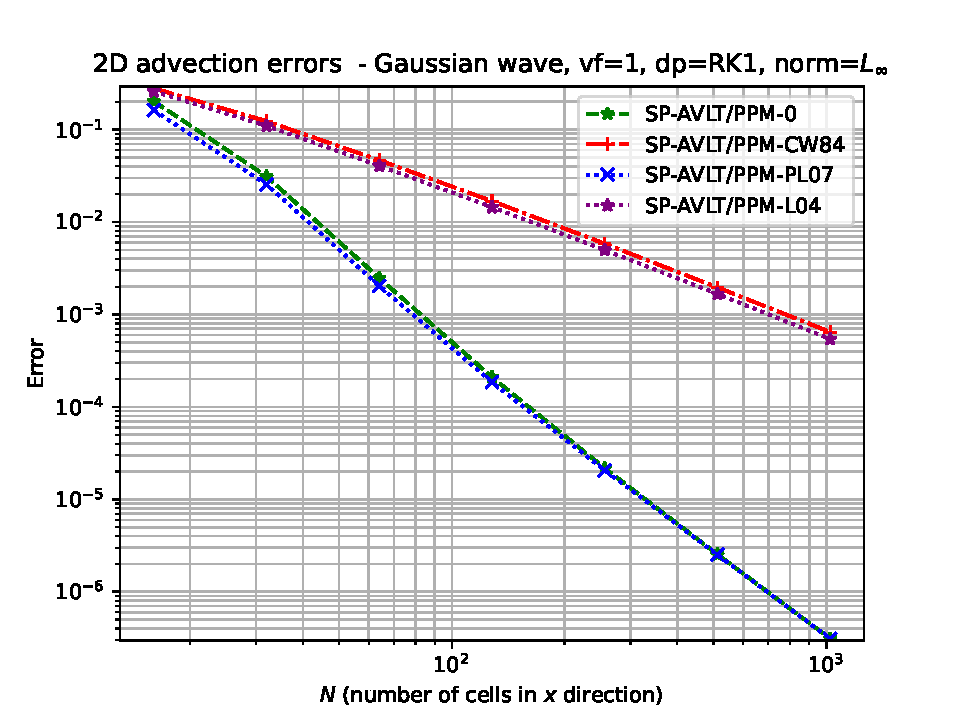
\includegraphics[width=1\linewidth]{2d_adv_tc2_ic2_vf1_dpRK1_normlinf_parabola_errors}
		\caption{Error.\label{chp3-sec-exp-adv1-error}}
	\end{subfigure}
	\begin{subfigure}{0.4\textwidth}
		\centering
		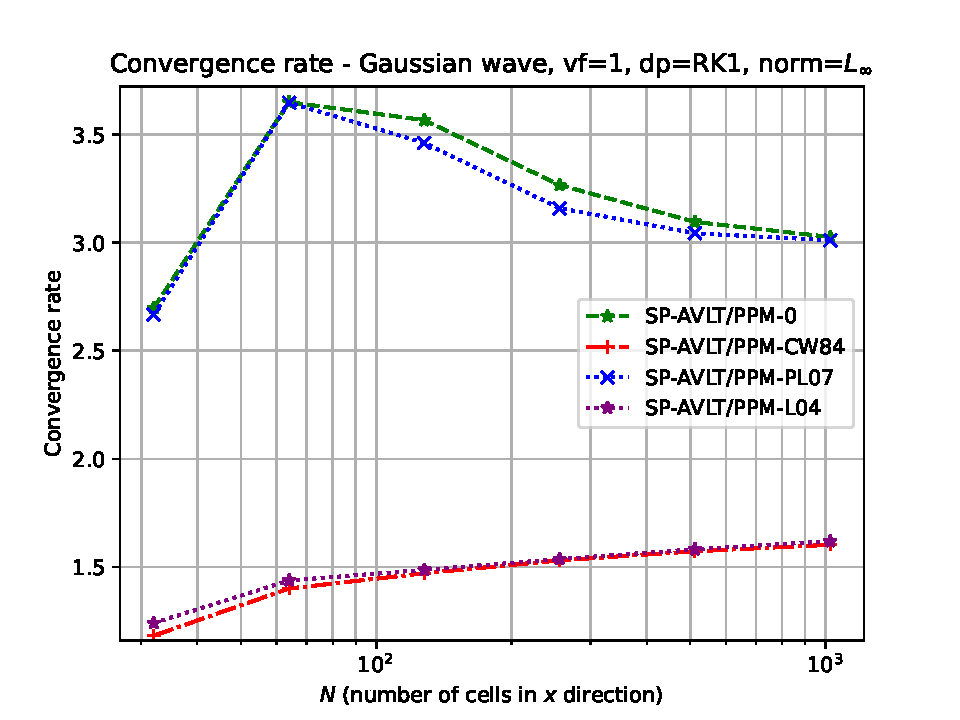
\includegraphics[width=1\linewidth]{2d_adv_tc2_ic2_vf1_dpRK1_normlinf_convergence_rate}
		\caption{Convergence rate.\label{chp3-sec-exp-adv1-CR}}
	\end{subfigure}
	\caption{Relative error convergence (a) and convergence rate (b) for PPM schemes with AVLT splitting
		applied to the advection equation using a constant velocity
		$\boldsymbol{u} = (0.2,-0.2)$, a CFL number equal to $0.8$, a final time equal to 5 time units
		and the initial condition given by Equation \eqref{chp3-ic1}.\label{chp3-sec-exp-adv1}}
\end{figure}

\begin{figure}[!htb]
	\centering
	\begin{subfigure}{0.4\textwidth}
		\centering
		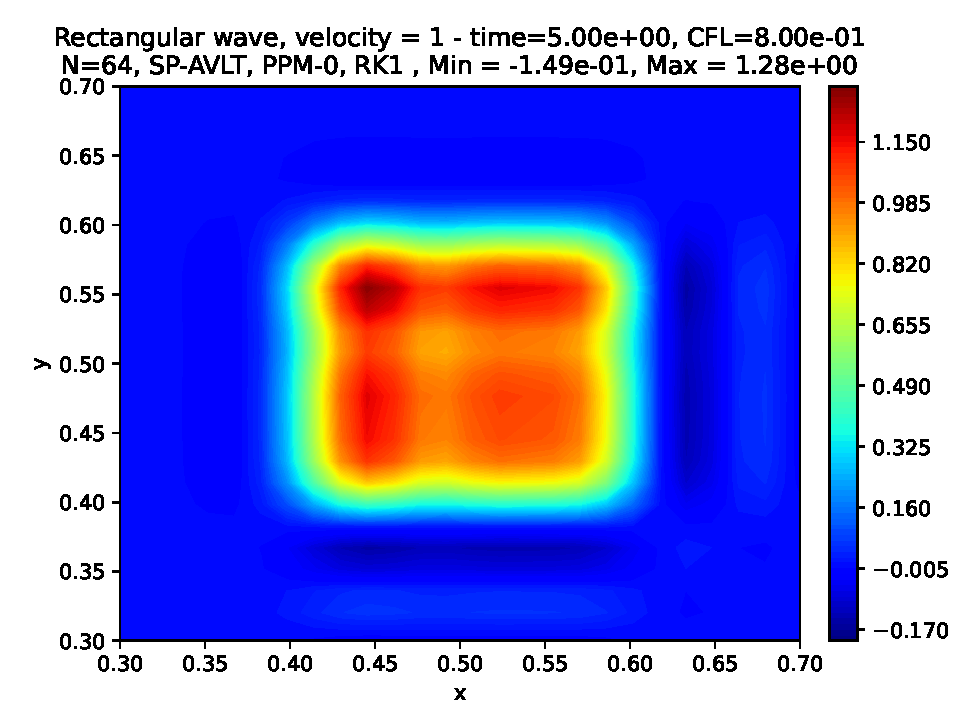
\includegraphics[width=1\linewidth]{2d_adv_tc1_ic3_vf1_t80_N64_SP-AVLT_PPM-0_RK1}
		\caption{PPM-0.\label{chp3-sec-exp-adv2-a}}
	\end{subfigure}
	\begin{subfigure}{0.4\textwidth}
		\centering
		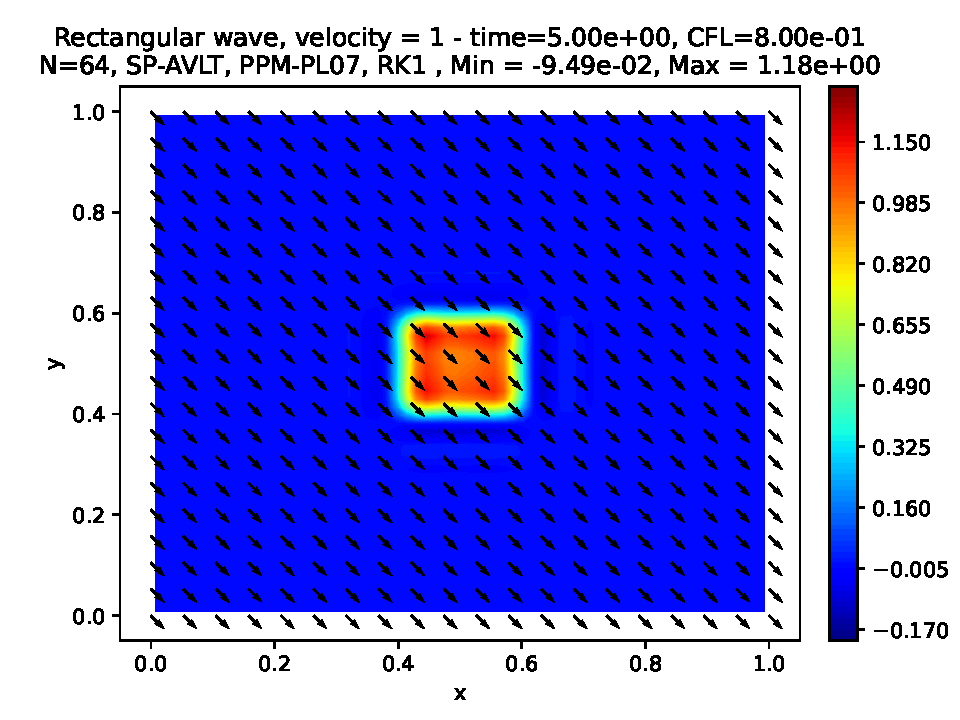
\includegraphics[width=1\linewidth]{2d_adv_tc1_ic3_vf1_t80_N64_SP-AVLT_PPM-PL07_RK1}
		\caption{PPM-PL07.\label{chp3-sec-exp-adv2-b}}
	\end{subfigure}
	
	\begin{subfigure}{0.4\textwidth}
		\centering
		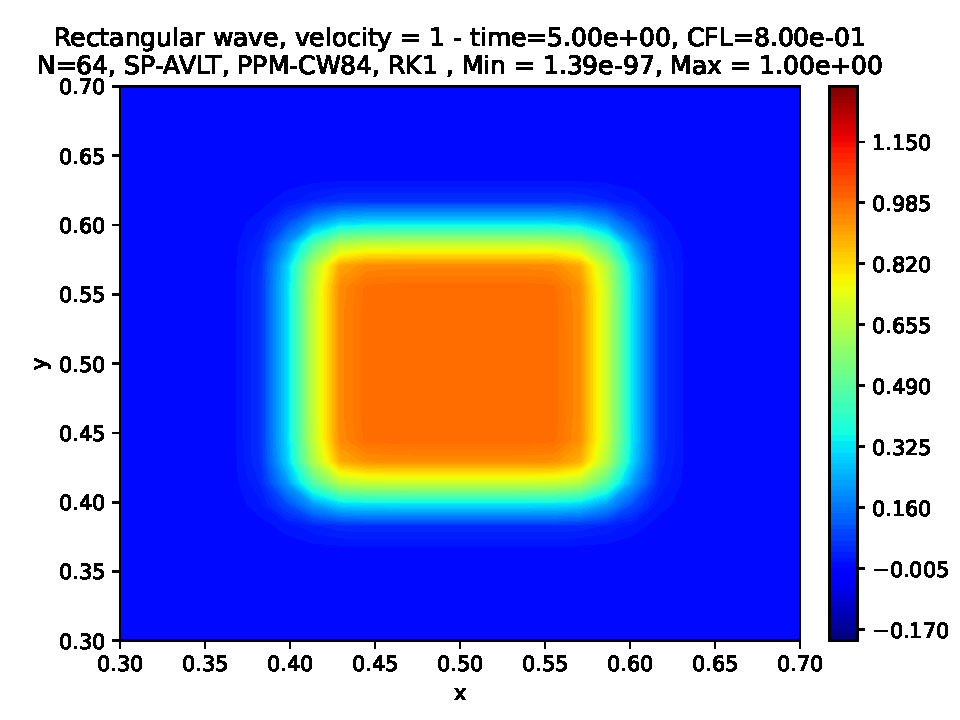
\includegraphics[width=1\linewidth]{2d_adv_tc1_ic3_vf1_t80_N64_SP-AVLT_PPM-CW84_RK1}
		\caption{PPM-CW84.\label{chp3-sec-exp-adv2-c}}
	\end{subfigure}
	\begin{subfigure}{0.4\textwidth}
		\centering
		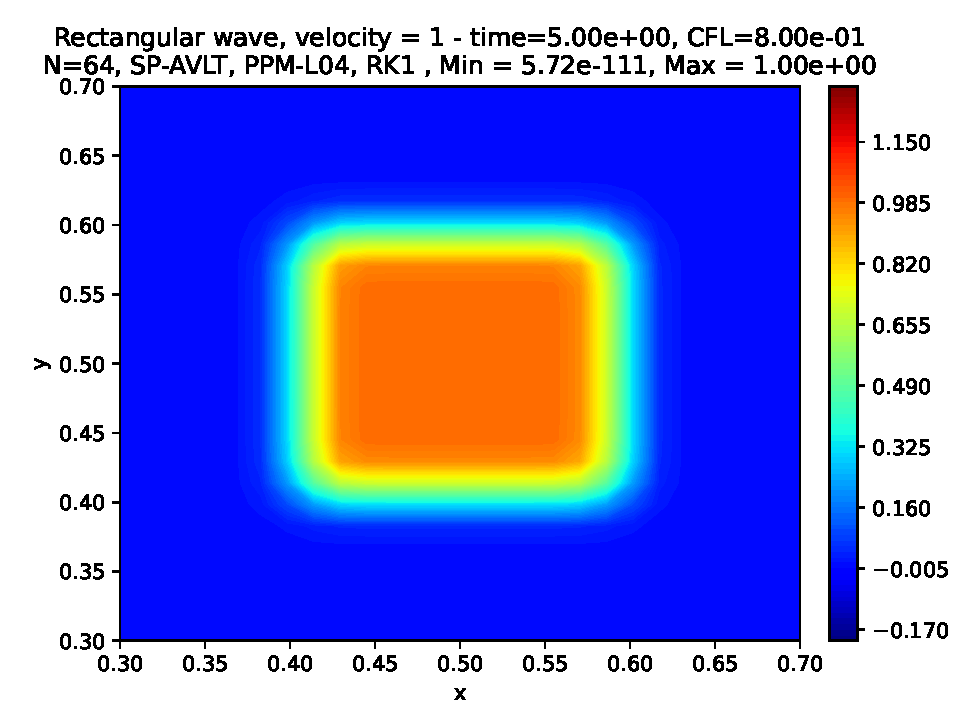
\includegraphics[width=1\linewidth]{2d_adv_tc1_ic3_vf1_t80_N64_SP-AVLT_PPM-L04_RK1}
		\caption{PPM-L04.\label{chp3-sec-exp-adv2-d}}
	\end{subfigure} 

	\begin{subfigure}{0.4\textwidth}
	\centering
	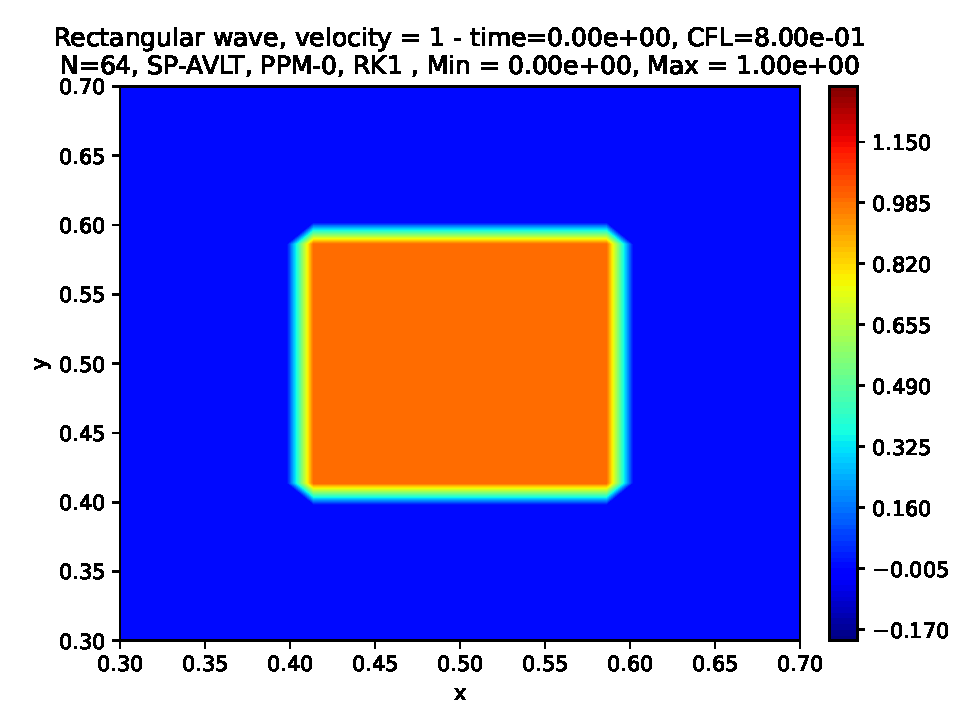
\includegraphics[width=1\linewidth]{2d_adv_tc1_ic3_vf1_t0_N64_SP-AVLT_PPM-0_RK1}
	\caption{Initial condition.\label{chp3-sec-exp-adv2-e}}
	\end{subfigure} 

	\caption{Linear advection experiment using a constant velocity equal to 
		$\boldsymbol{u} = (0.2,-0.2)$,
		a CFL number equal to $0.8$, $N=M=64$, and the initial condition is given by Equation \eqref{chp3-ic2}.
		We use the schemes PPM-0, PPM-PL07, PPM-CW84 and PPM-L04 with AVLT splitting.
		These figures show the advected profile after 5 time units (one time period).
		The initial condition is shown in (e).
		\label{chp3-sec-exp-adv2}}
\end{figure}

The  exact solution of Problem \ref{chp3-sec2-prob1} in this case
is $q_0(x-ut)$ for both $q_0$. 
Since the velocity field is constant, all the splitting schemes introduce in
Section \ref{sec-dsplit} are the same, hence we are just going to consider the AVLT
splitting. Besides that, it is easy to see that the Lie-Trotter splitting is exact in this case
(cf. eg. \cite[p.~ 202-203]{leveque:1990}).
For 1D schemes, we use the RK1 to compute the departure point,
since this scheme is exact if the velocity is constant. 

The conclusions for the constant velocity tests are very similar to the 1D tests from Section \ref{chp2-sec-numerical-exp-1}.
In fact, the error and convergence rate (Figure \ref{chp3-sec-exp-adv1}) for the Gaussian
profile is very similar to the one-dimensional case (Figure \ref{chp2-sec-exp-adv2-2}). This behavior is due to the fact of 
no splitting error is introduced when the velocity is constant. From 
Figure \ref{chp3-sec-exp-adv2}, we can see that the AVLT splitting preserves the monotonicity
when we use the monotonic 1D schemes PPM-CW84 and PPM-L04. For the non-monotonic schemes, we 
observe as in Figure \ref{chp2-sec-exp-adv3} that PPM-PL07 produces less numerical dispersion than PPM-0.

\subsection{Linear advection equation with variable velocity simulations}
For variable velocity testing, we consider two Gaussian hills given by:
\begin{align}
	\begin{split}
	\label{chp3-ic3}
	q_0(x,y) = &\exp(-10\cos^2 (2\pi (x-0.1))\exp(-10\cos^2 (2\pi y)) + \\
			   &\exp(-10\cos^2 (2\pi (x+0.1))) \exp(-10\cos^2 (2\pi y)),
	\end{split}
\end{align}
defined in $[0,1] \times [0,1]$, whose graph is shown in Figure \ref{chp3-sec-exp-adv3-ic}.
\begin{figure}[!htb]
	\begin{subfigure}{0.45\textwidth}
		\centering
		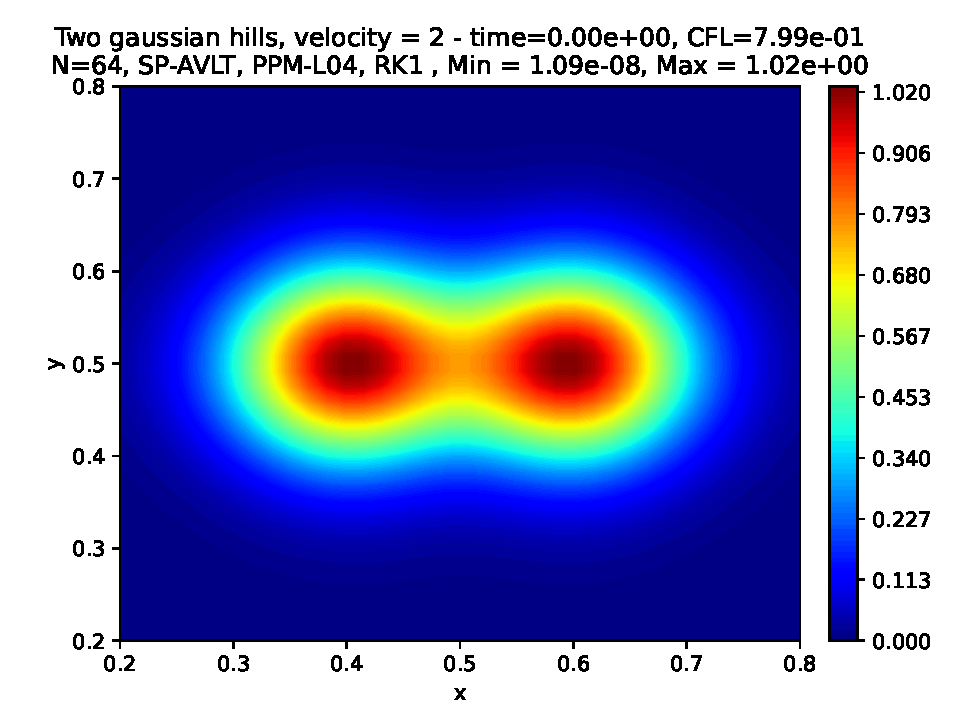
\includegraphics[width=1\linewidth]{2d_adv_tc1_ic4_vf2_t0_N64_SP-AVLT_PPM-L04_RK1}
		\caption{Initial condition from Equation \eqref{chp3-ic3}.\label{chp3-sec-exp-adv3-ic}}
	\end{subfigure} 
\end{figure}

We consider the velocity proposed by \citet{nair:2010}:
\begin{equation}
	\label{chp3-vf1}
	\begin{cases}
		u(x,y,t) &=  \sin(\pi x)^2\sin(2\pi y)\cos\big(\frac{\pi t}{T}\big),\\
		v(x,y,t) &= -\sin(\pi y)^2\sin(2\pi x)\cos\big(\frac{\pi t}{T}\big),
	\end{cases}
\end{equation}
where $T=5$. We also consider the Cartesian version of the deformational flow test case on the sphere from \citet{nair:2010}
proposed by \citet{chen:2017}. The velocity is given by:
\begin{equation}
	\label{chp3-vf2}
	\begin{cases}
		u(x,y,t) &= c\frac{\pi}{L_y}\sin^2(\alpha_1)(2\cos(\alpha_2)\sin(\alpha_2))(\cos(\alpha_3)) - \frac{L_x}{T},\\
		v(x,y,t) &= \frac{-c}{\pi}\frac{2\pi}{L_x}(2\sin(\alpha_1)\cos(\alpha_1)\cos^2(\alpha_2))\cos(\alpha_3),
	\end{cases}
\end{equation}
where $L_x = 2\pi$, $L_y = \pi$, $T=5$, $c = \frac{10}{T}(\frac{L_x}{2\pi})^2$, $\alpha_1 = 2\pi\big(\frac{X}{L_x}-\frac{t}{T}\big)$, $\alpha_2 = \frac{\pi Y}{L_y}$,
$\alpha_3 =\frac{\pi t}{T}$,  $X = -\pi + 2\pi x $, $Y =-\frac{\pi}{2} +\pi y$. 
\citet{chen:2017} uses periodic boundary conditions in the $x-$direction and zero-gradient in the $y-$direction.
We shall employ biperiodic boundary conditions to simplify the problem.
Both velocity fields are divergence-free and they deform the initial condition after 5 time units the scalar field
returns to its initial position and shape, therefore we can compute the error.

\newpage
\begin{figure}[!htb]
	\centering
	\begin{subfigure}{0.4\textwidth}
		\centering
		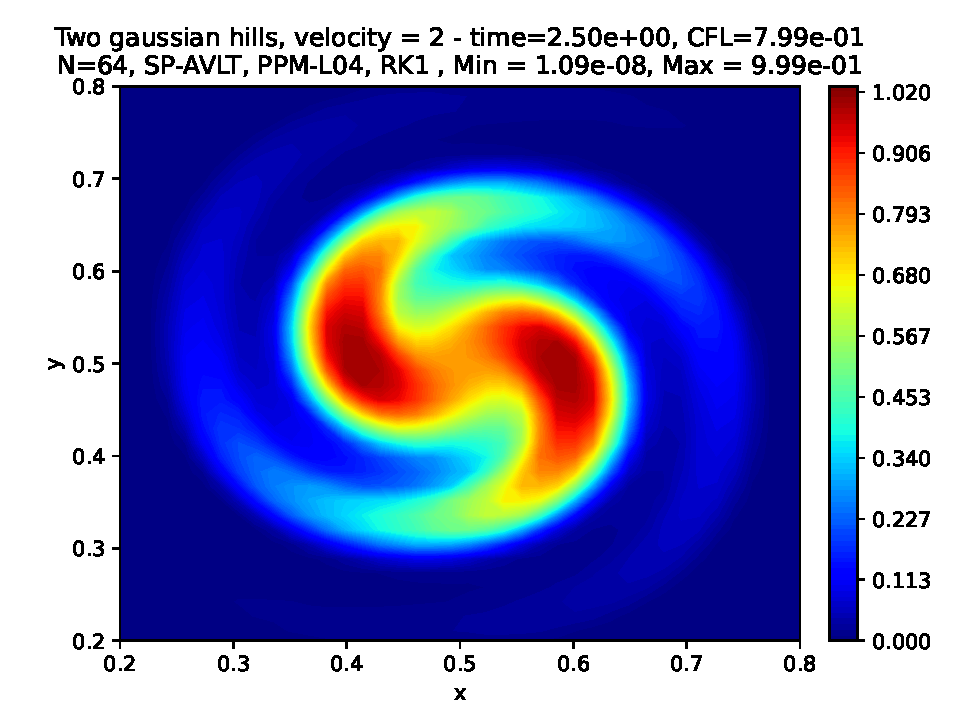
\includegraphics[width=1\linewidth]{2d_adv_tc1_ic4_vf2_t200_N64_SP-AVLT_PPM-L04_RK1}
		\caption{AVLT splitting at $t=2.5$.\label{chp3-sec-exp-adv3-a}}
	\end{subfigure}
	\begin{subfigure}{0.4\textwidth}
		\centering
		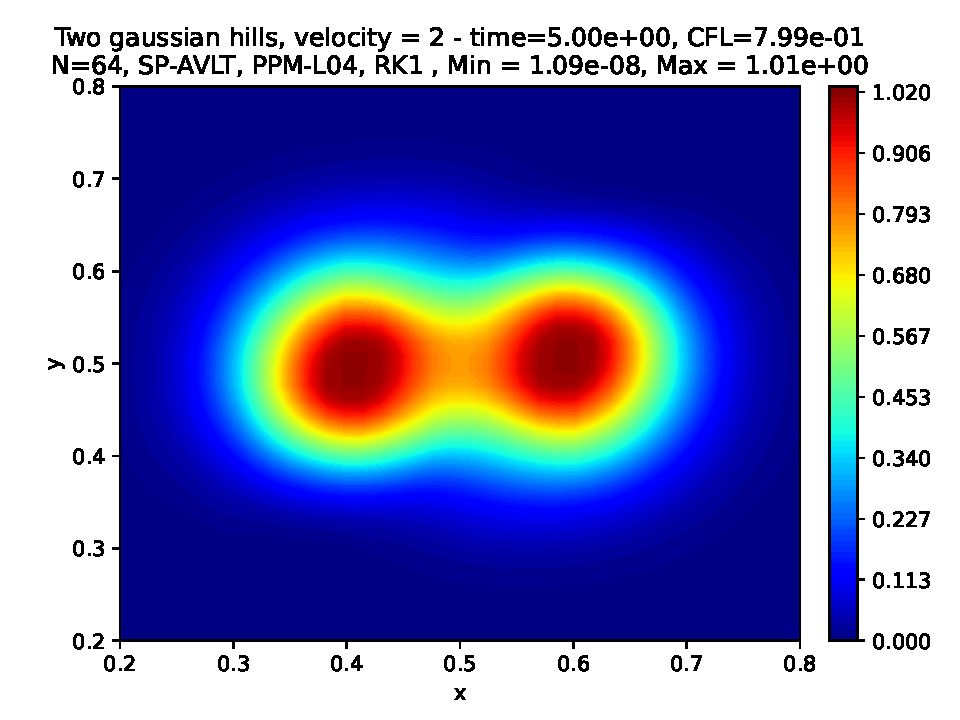
\includegraphics[width=1\linewidth]{2d_adv_tc1_ic4_vf2_t400_N64_SP-AVLT_PPM-L04_RK1}
		\caption{AVLT splitting at $t=5$.\label{chp3-sec-exp-adv3-b}}
	\end{subfigure}
	
	\begin{subfigure}{0.4\textwidth}
		\centering
		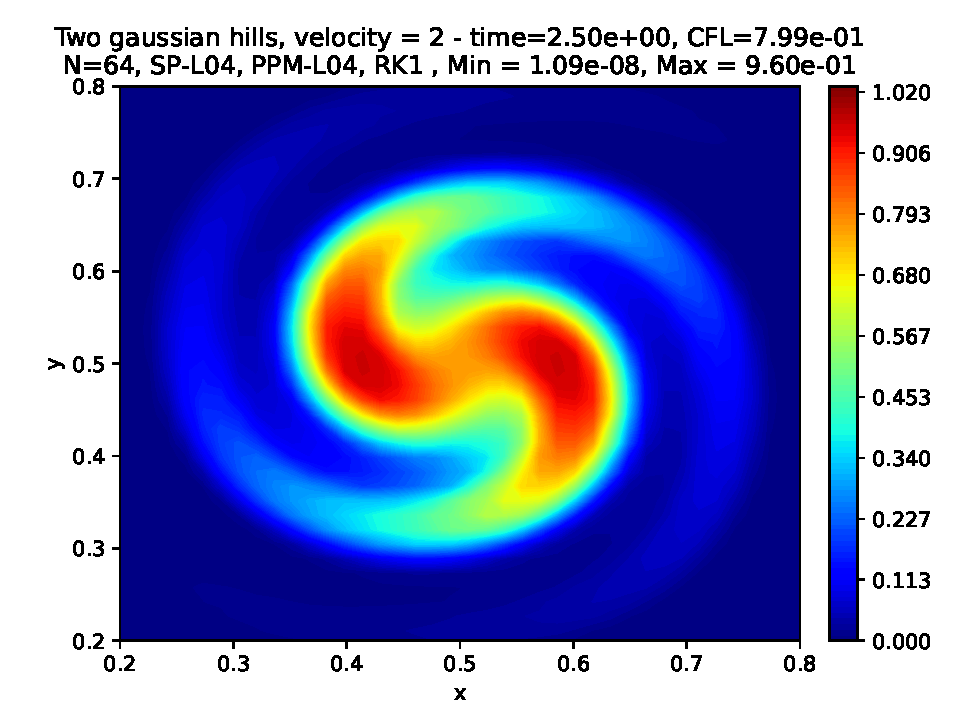
\includegraphics[width=1\linewidth]{2d_adv_tc1_ic4_vf2_t200_N64_SP-L04_PPM-L04_RK1}
		\caption{L04 splitting at $t=2.5$.\label{chp3-sec-exp-adv3-c}}
	\end{subfigure}
	\begin{subfigure}{0.4\textwidth}
		\centering
		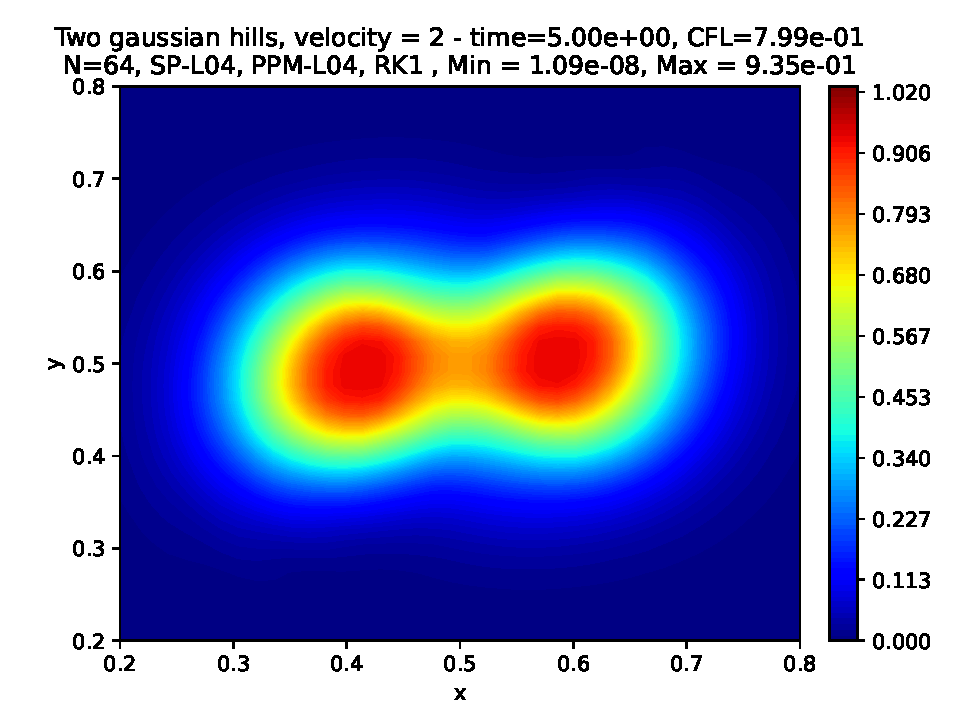
\includegraphics[width=1\linewidth]{2d_adv_tc1_ic4_vf2_t400_N64_SP-L04_PPM-L04_RK1}
		\caption{L04 splitting at $t=5$.\label{chp3-sec-exp-adv3-d}}
	\end{subfigure} 

	\begin{subfigure}{0.4\textwidth}
		\centering
		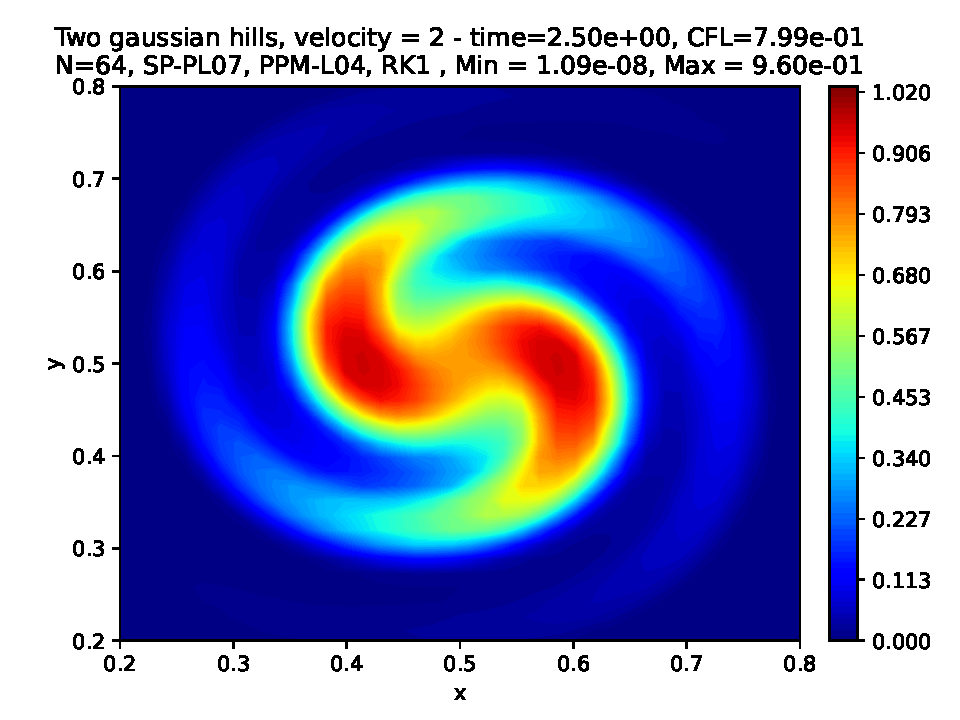
\includegraphics[width=1\linewidth]{2d_adv_tc1_ic4_vf2_t200_N64_SP-PL07_PPM-L04_RK1}
		\caption{PL07 splitting at $t=2.5$.\label{chp3-sec-exp-adv3-e}}
	\end{subfigure}
	\begin{subfigure}{0.4\textwidth}
		\centering
		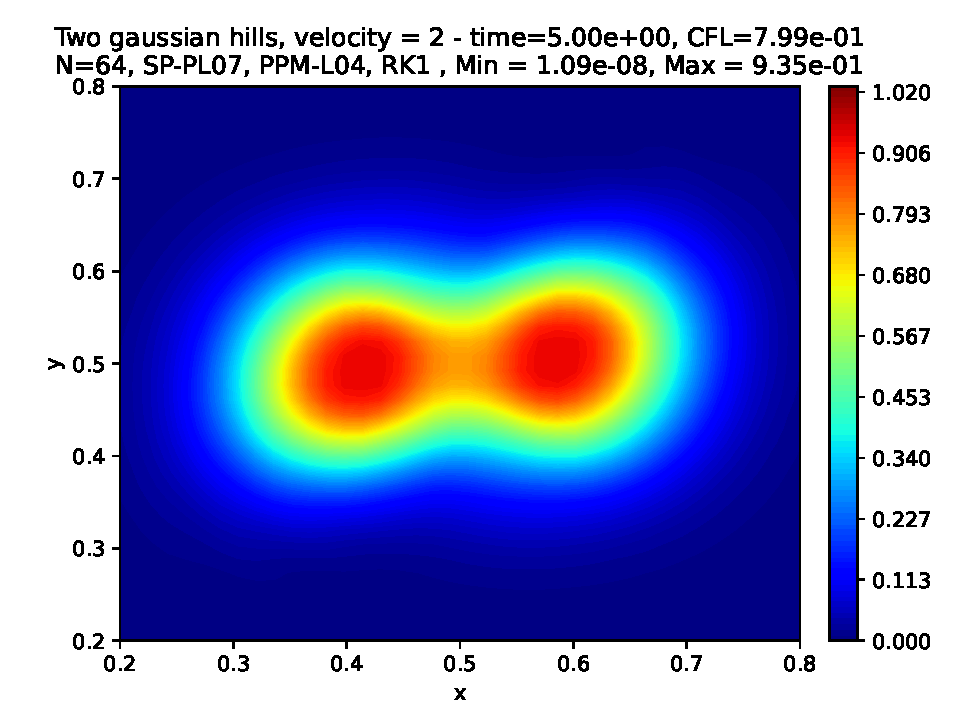
\includegraphics[width=1\linewidth]{2d_adv_tc1_ic4_vf2_t400_N64_SP-PL07_PPM-L04_RK1}
		\caption{PL07 splitting at $t=5$.\label{chp3-sec-exp-adv3-f}}
	\end{subfigure} 
	
	\caption{Linear advection experiment using the velocity from Equation \eqref{chp3-vf1},
		a CFL number equal to $0.8$, $N=M=64$, and the initial condition is given by Equation \eqref{chp3-ic3}.
		We use the scheme PPM-L04 with AVLT  (a and b), L04 (c and d) and PL07 (e and f) splitting and RK1 departure point scheme.
		These figures show the advected profile after 2.5 (left) and 5  (right) time units (one time period).
		\label{chp3-sec-exp-adv3}}
\end{figure}

In Figure \ref{chp3-sec-exp-adv3} we depict the results obtained using the two Gaussian hills and the velocity field from
Equation \eqref{chp3-vf2} using the PPM-L04 with AVLT, L04, and PL07 splitting and RK1 as the departure point scheme.
We can observe how the scalar field has deformed and returns to its initial position. However, we can notice
that the PL07 and L04 splitting are more diffusive than the AVLT splitting when we look at the solution after 5 time units in 
Figure \ref{chp3-sec-exp-adv3}.
Employing the RK1 scheme and also considering the PPM-PL07 scheme, 
from Figure \ref{chp3-sec-exp-adv5} and Figure \ref{chp3-sec-exp-adv6} we observe that the AVLT has the larger error considering and
all schemes have first-order of accuracy (Figure \ref{chp3-sec-exp-adv6-error1}).
However, when we use the RK3 scheme, the most accurate schemes are obtained with AVLT with PPM-L07,
which reaches third-order (Figure \ref{chp3-sec-exp-adv6-error2}), despite AVLT being second-order, followed by AVLT with PPM-L04 (Figure \ref{chp3-sec-exp-adv5-error2}).
The other schemes seem only to not improve but get a larger error using RK3. Therefore, we conclude that the L04 and PL07 splitting 
introduce a first-order error. Furthermore, these schemes do not seem to differ one from the other.
\begin{figure}[!htb]
	\centering
	\begin{subfigure}{0.4\textwidth}
		\centering
		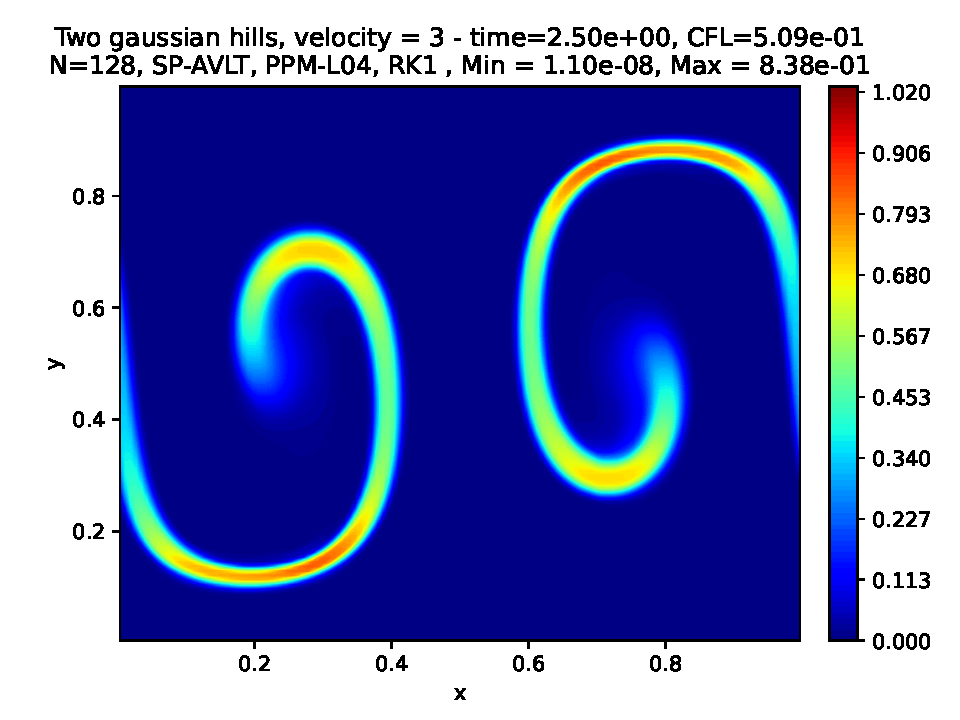
\includegraphics[width=1\linewidth]{2d_adv_tc1_ic4_vf3_t400_N128_SP-AVLT_PPM-L04_RK1}
		\caption{AVLT splitting at $t=2.5$.\label{chp3-sec-exp-adv4-a}}
	\end{subfigure}
	\begin{subfigure}{0.4\textwidth}
		\centering
		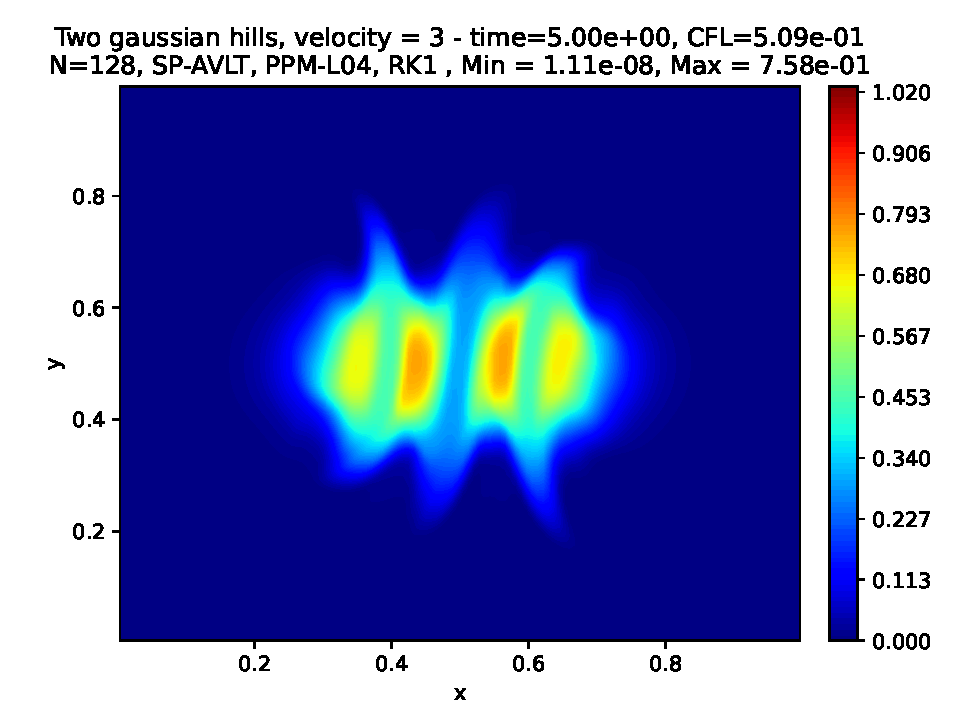
\includegraphics[width=1\linewidth]{2d_adv_tc1_ic4_vf3_t800_N128_SP-AVLT_PPM-L04_RK1}
		\caption{AVLT splitting at $t=5$.\label{chp3-sec-exp-adv4-b}}
	\end{subfigure}
	
	\begin{subfigure}{0.4\textwidth}
		\centering
		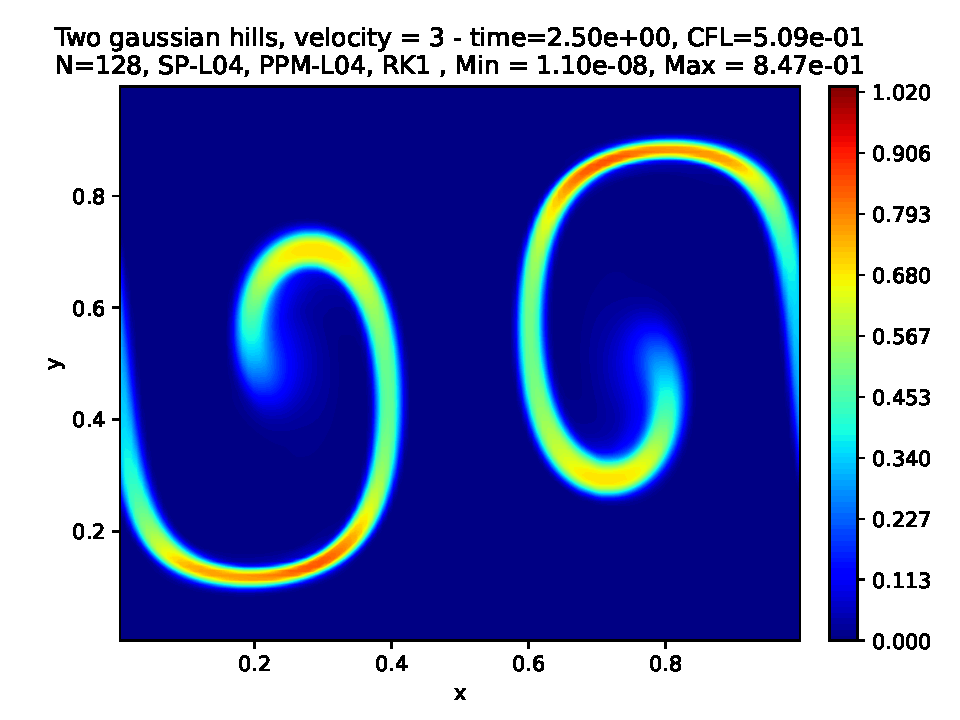
\includegraphics[width=1\linewidth]{2d_adv_tc1_ic4_vf3_t400_N128_SP-L04_PPM-L04_RK1}
		\caption{L04 splitting at $t=2.5$.\label{chp3-sec-exp-adv4-c}}
	\end{subfigure}
	\begin{subfigure}{0.4\textwidth}
		\centering
		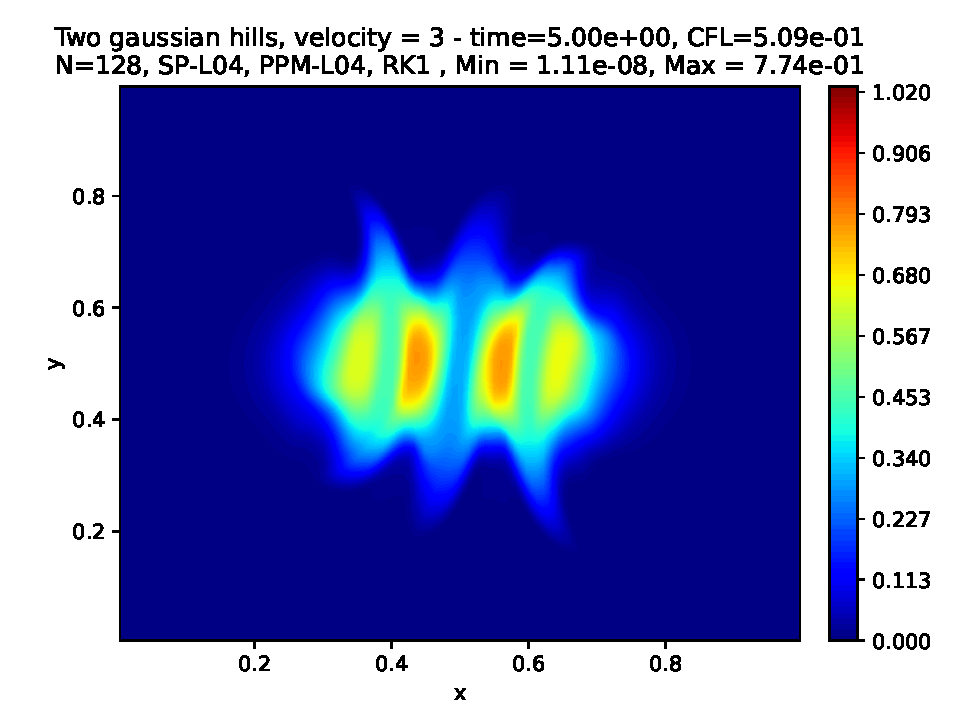
\includegraphics[width=1\linewidth]{2d_adv_tc1_ic4_vf3_t800_N128_SP-L04_PPM-L04_RK1}
		\caption{L04 splitting at $t=5$.\label{chp3-sec-exp-adv4-d}}
	\end{subfigure} 
	
	\begin{subfigure}{0.4\textwidth}
		\centering
		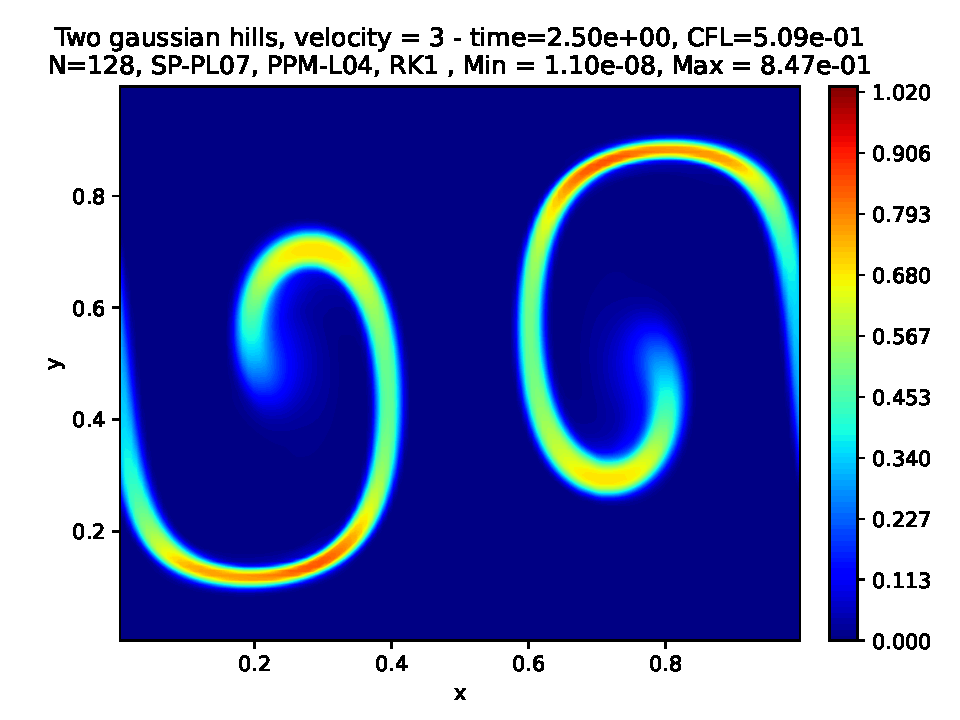
\includegraphics[width=1\linewidth]{2d_adv_tc1_ic4_vf3_t400_N128_SP-PL07_PPM-L04_RK1}
		\caption{PL07 splitting at $t=2.5$.\label{chp3-sec-exp-adv4-e}}
	\end{subfigure}
	\begin{subfigure}{0.4\textwidth}
		\centering
		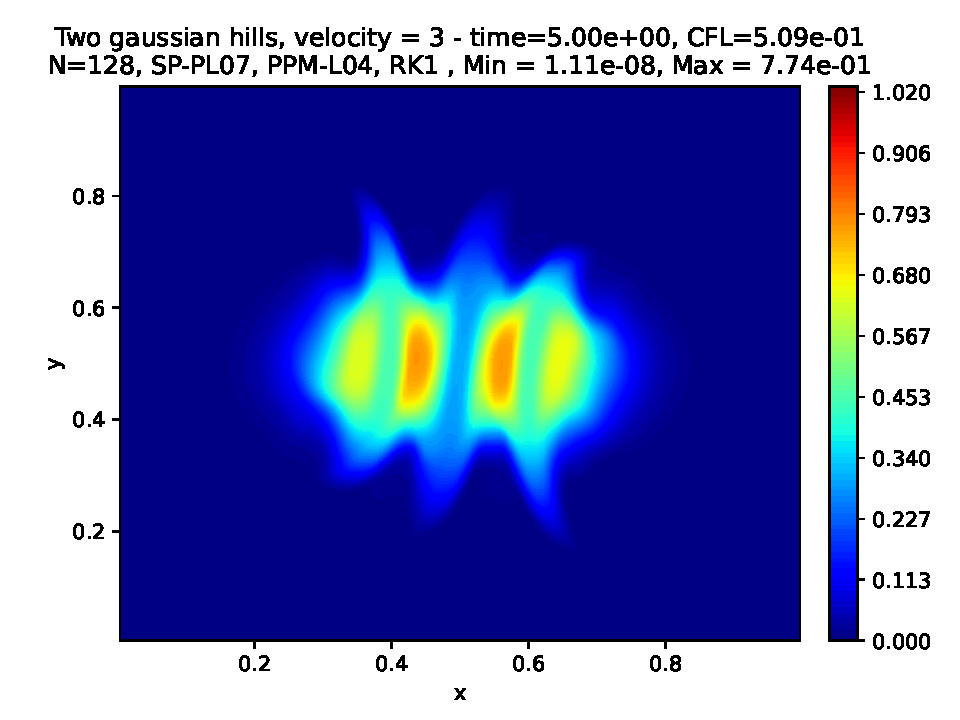
\includegraphics[width=1\linewidth]{2d_adv_tc1_ic4_vf3_t800_N128_SP-PL07_PPM-L04_RK1}
		\caption{PL07 splitting at $t=5$.\label{chp3-sec-exp-adv4-f}}
	\end{subfigure} 
	
	\caption{Similar to Figure \ref{chp3-sec-exp-adv4} but using the velocity from Equation \eqref{chp3-vf2} and $N=128$.
		\label{chp3-sec-exp-adv4}}
\end{figure}

In Figure \ref{chp3-sec-exp-adv4} we depict the results using the same setup and schemes as before but using the velocity from
Equation \eqref{chp3-vf2}. 
As in the previous test, we see the velocity deformarting the Gaussian hills.
Again the PL07 and L04 schemes produce almost the same results, however, in contrast with previous test, 
they are less diffusive than the AVLT.
From Figure \ref{chp3-sec-exp-adv7-error1},  notice that, when using the RK1 schemes, 
the PL07 and L04 schemes are slightly more accurate than AVLT for the 1D PPM-PL07 schemes.
All these schemes reaches a converge-order superior to two (Figure \ref{chp3-sec-exp-adv8-error1}).
When we use the 1D scheme PPM-L04, all the splitting method are very similar,
regardless the departure point scheme.
However, when use the RK3 schemes, the AVLT is the most accurate and reaches third-order (Figure \ref{chp3-sec-exp-adv8-error2}).

\begin{figure}[!htb]
	\centering
	\begin{subfigure}{0.45\textwidth}
		\centering
		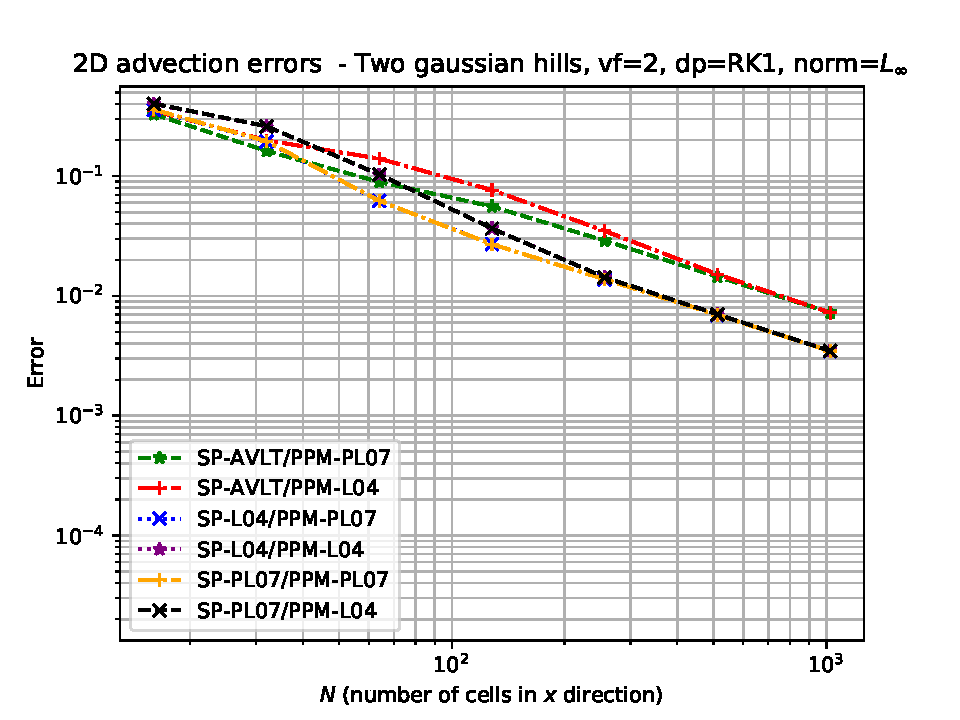
\includegraphics[width=1\linewidth]{2d_adv_tc2_ic4_vf2_dpRK1_normlinf_parabola_errors}
		\caption{RK1.\label{chp3-sec-exp-adv5-error1}}
	\end{subfigure}
	\begin{subfigure}{0.45\textwidth}
		\centering
		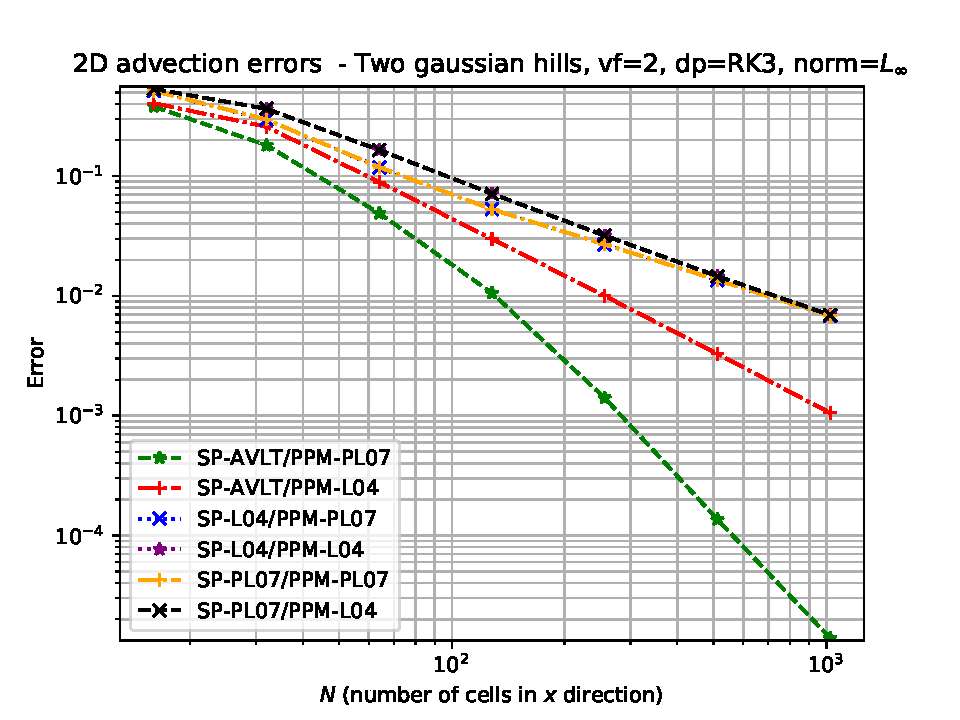
\includegraphics[width=1\linewidth]{2d_adv_tc2_ic4_vf2_dpRK3_normlinf_parabola_errors}
		\caption{RK3.\label{chp3-sec-exp-adv5-error2}}
	\end{subfigure}
	\caption{Convergence of the error for the schemes
	PPM-PL07and PPM-L04 with AVLT/L04/PL07/ splitting
	applied to the linear advection problem using a velocity from Equation
	a CFL number equal to $0.8$, a final time of integration equal to 5 time units
	and the initial condition given by Equation \eqref{chp3-ic1}.
	The departure points are computed using the RK1 (left) and RK3 (right) schemes.\label{chp3-sec-exp-adv5}}
\end{figure}

\begin{figure}[!htb]
	\centering
	\begin{subfigure}{0.45\textwidth}
		\centering
		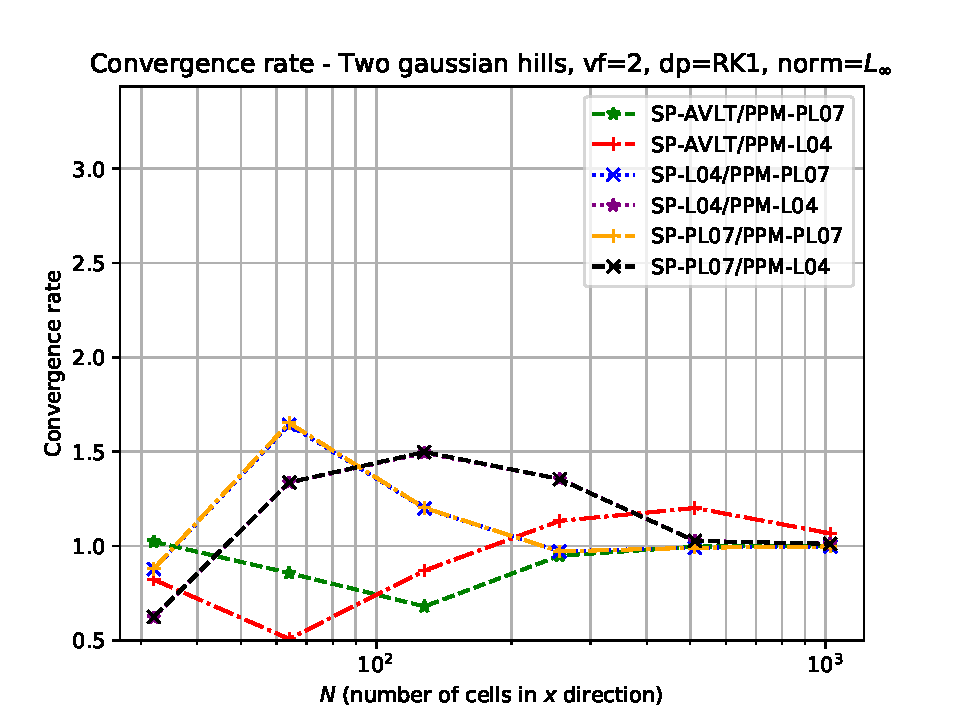
\includegraphics[width=1\linewidth]{2d_adv_tc2_ic4_vf2_dpRK1_normlinf_convergence_rate}
		\caption{RK1.\label{chp3-sec-exp-adv6-error1}}
	\end{subfigure}
	\begin{subfigure}{0.45\textwidth}
		\centering
		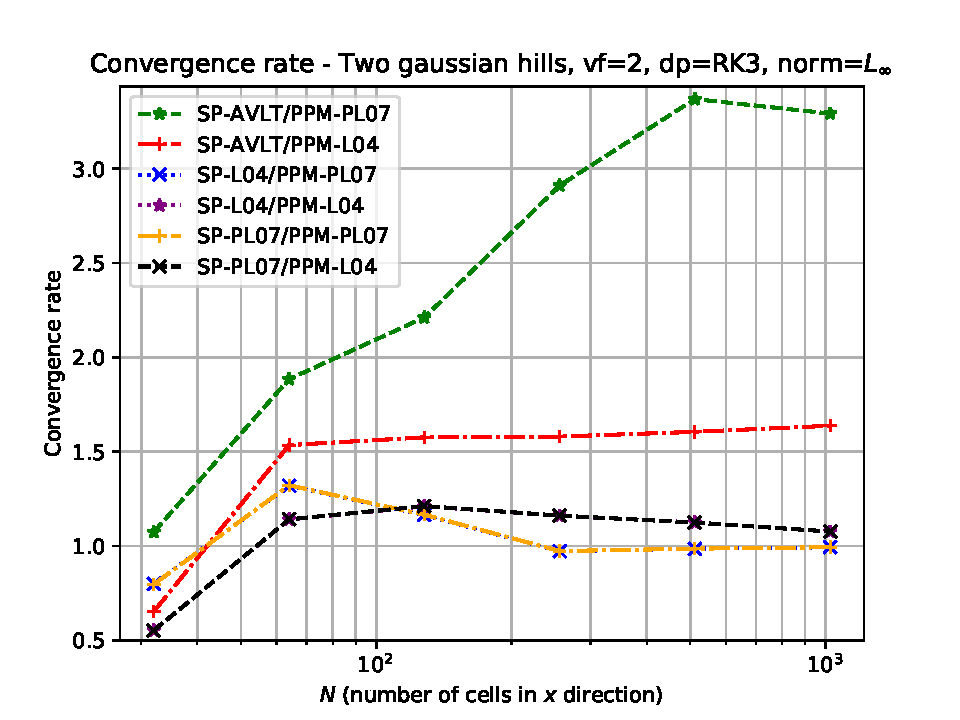
\includegraphics[width=1\linewidth]{2d_adv_tc2_ic4_vf2_dpRK3_normlinf_convergence_rate}
		\caption{RK3.\label{chp3-sec-exp-adv6-error2}}
	\end{subfigure}
	\caption{Similar to Figure \ref{chp3-sec-exp-adv5} but considering the convergence rate.\label{chp3-sec-exp-adv6}}
\end{figure}


\begin{figure}[!htb]
	\centering
	\begin{subfigure}{0.45\textwidth}
		\centering
		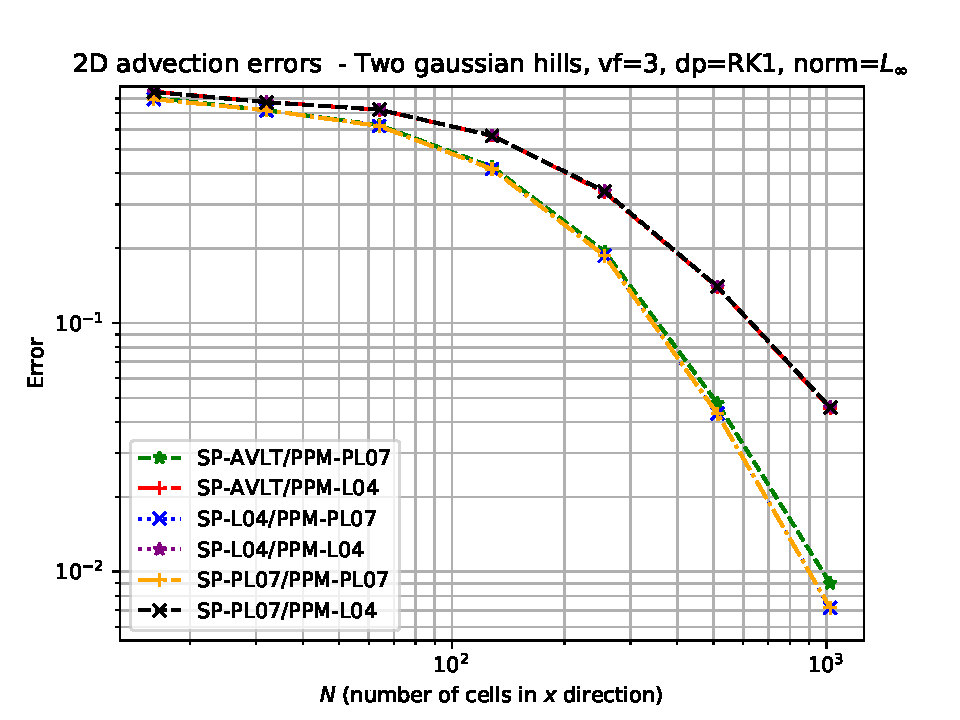
\includegraphics[width=1\linewidth]{2d_adv_tc2_ic4_vf3_dpRK1_normlinf_parabola_errors}
		\caption{RK1.\label{chp3-sec-exp-adv7-error1}}
	\end{subfigure}
	\begin{subfigure}{0.45\textwidth}
		\centering
		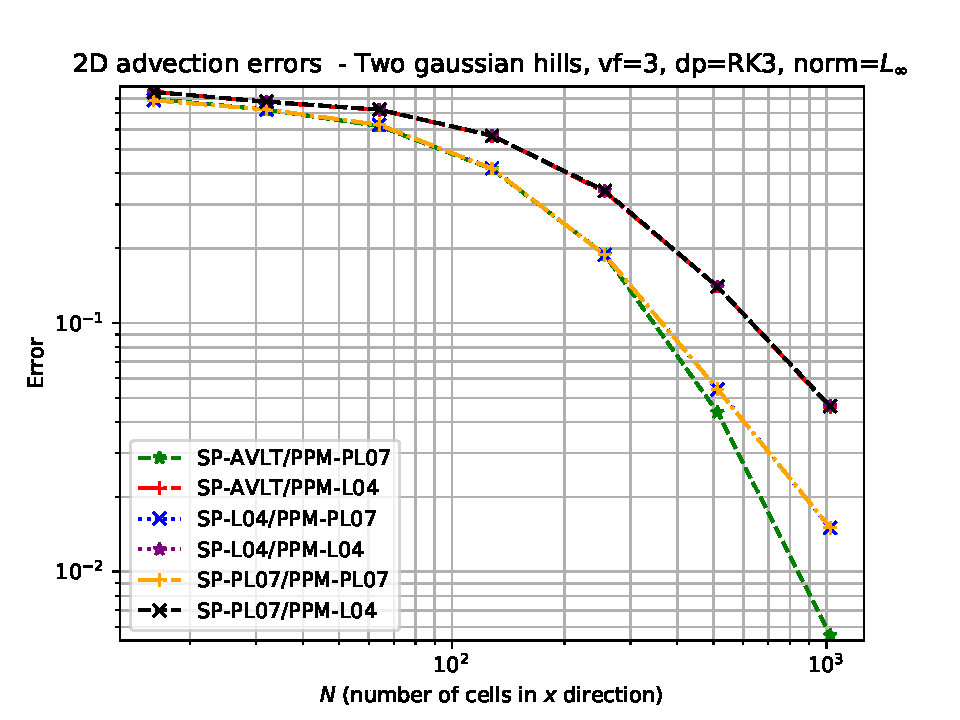
\includegraphics[width=1\linewidth]{2d_adv_tc2_ic4_vf3_dpRK3_normlinf_parabola_errors}
		\caption{RK3.\label{chp3-sec-exp-adv7-error2}}
	\end{subfigure}
	\caption{Similar to Figure \ref{chp3-sec-exp-adv5} but using the velocity from Equation \eqref{chp3-vf2}.\label{chp3-sec-exp-adv7}}
\end{figure}

\begin{figure}[!htb]
	\centering
	\begin{subfigure}{0.45\textwidth}
		\centering
		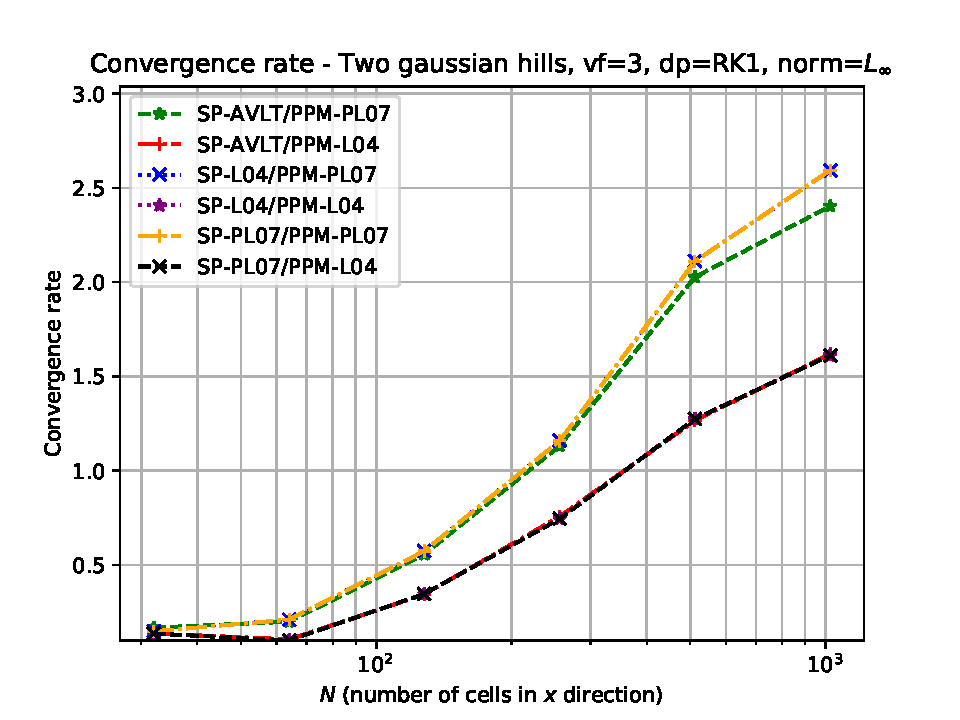
\includegraphics[width=1\linewidth]{2d_adv_tc2_ic4_vf3_dpRK1_normlinf_convergence_rate}
		\caption{RK1.\label{chp3-sec-exp-adv8-error1}}
	\end{subfigure}
	\begin{subfigure}{0.45\textwidth}
		\centering
		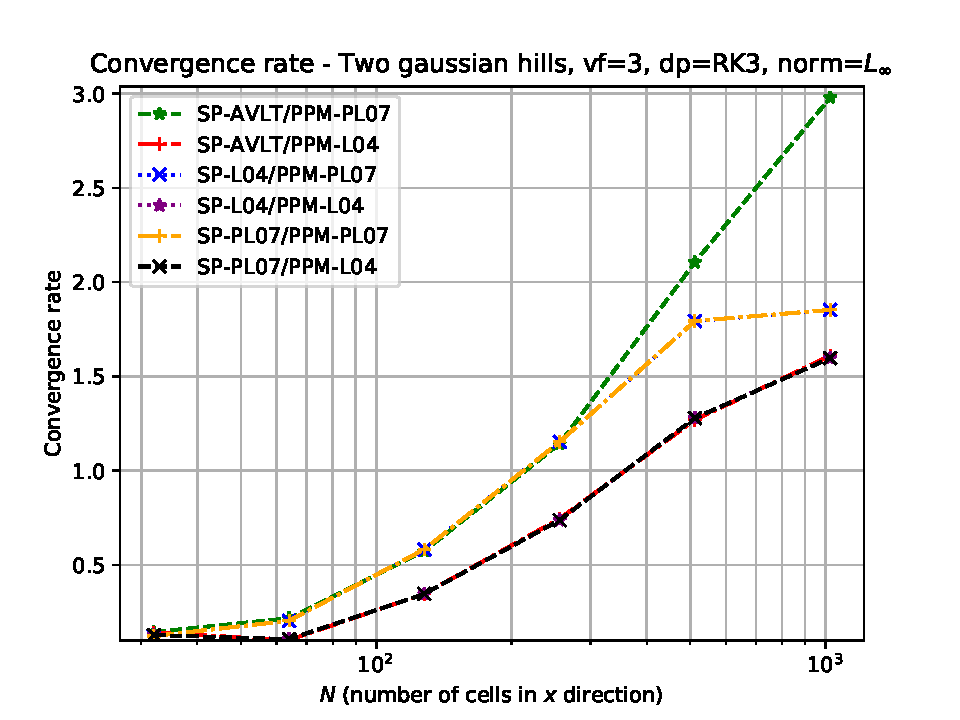
\includegraphics[width=1\linewidth]{2d_adv_tc2_ic4_vf3_dpRK3_normlinf_convergence_rate}
		\caption{RK3.\label{chp3-sec-exp-adv8-error2}}
	\end{subfigure}
	\caption{Similar to Figure \ref{chp3-sec-exp-adv6} but using the velocity from Equation   \eqref{chp3-vf2}.\label{chp3-sec-exp-adv8}}
\end{figure}

\break
\section{Concluding remarks}
In this Chapter, we introduced the dimension-splitting method which replaces the solution
of the 2D advection equation by the solution of multiples 1D advection equations.
The average of two Lie-Trotter splitting. which is second-order accurate, was modified to ensure the preservation of a constant scalar field
with a divergence-free velocity, which the classical averaging Lie-Trotter splitting lacks, following
the methodology used in FV3.

From the constant velocity simulations, we conclude that all the splitting schemes are equal 
and they do not introduce any splitting error. In fact, they are exact. We could observe
that all conclusion for the 1D simulations were wit in the 2D case, with mass conservation
and monotonicity  being respected in the 2D case whenever we employ it in the 1D subproblems.

For variable velocity simulations, we investigated two deformation test cases.
We observed that all splitting schemes preserved the monotonicity.
The schemes PL07 and L04 yields very similar results and they introduced a first-order error,
which was observed when we employed the RK3 scheme to compute the departure point.
In this case, the AVLT reached third-order of accuracy, which is better than expected since this scheme
is only second-order. Therefore, we can conclude that a more accurate departure point calculation
benefits more the AVLT splitting. However, when using a first-order departure point computation, the splitting schemes
PL07 and L04 produced slightly smaller errors.